%%
%%  Department of Electrical, Electronic and Computer Engineering.
%%  EPR400/2 Final Report - Main File.
%%  Copyright (C) 2011-2021 University of Pretoria.
%%

\documentclass{epr400}

%% EDIT: Replace the following with your information.
\eprtitle{Design and implementation of a dual WiFI/cellular linked
smart energy meter}
\eprcode{EPR400}
\eprcandidatename{J Wagener}
\eprstudentnumber{16056214}
\eprdate{November 2022}
\eprsupervisor{Dr. JH van Wyk}
\eprcopynum{Electronic copy}

\begin{document}

\tikzstyle{terminator} = [rectangle, draw, text centered, rounded corners, minimum height=2em]
\tikzstyle{process} = [rectangle, draw, text centered, minimum height=2em]
\tikzstyle{decision} = [diamond, draw, text centered, minimum height=2em]
\tikzstyle{data}=[trapezium, draw, text centered, trapezium left angle=60, trapezium right angle=120, minimum height=2em]
\tikzstyle{connector} = [draw, -latex']

%% Generate the required title page.
\maketitlepage

%% --- PART 1 ------------------------------------------------------------

\pagestyle{plain}
\pagenumbering{roman}

\eprsec{Part 1. Preamble}

\vspace*{0.5cm}

%% Import the required preamble pages.
%%
%%  Department of Electrical, Electronic and Computer Engineering.
%%  EPR400/2 Final Report - Preamble.
%%  Copyright (C) 2011-2021 University of Pretoria.
%%
This report was compiled to outline the research and production process of developing a non-intrusive load detection energy meter for appliance identification (this device being my final year project submission).
\\[2ex]
\textit{Project proposal and technical documentation} \newline
This main report contains an unaltered copy of the approved Project Proposal (as Part 2 of the report).

Technical documentation appears in Part 4 (Appendix).

All the code that I developed appears as a separate submission on the AMS.
\\[2ex]
\textit{Project history} \newline
The work of Gouhua \emph{et al} in \cite{RN39} was used as a basis and point of departure for this project. However, though the method of identification used is the same as that of Gouha \emph{et al}, the implementation of their work in the creation of the device appears to be unprecedented and original. This project makes extensive use of existing algorithms on decision trees - many of which were adapted from \cite{jauregui_2022}, though other authors' work was also relied upon (and appropriately cited).
\\[2ex]
I reused FFT code from a library and did not develop this myself.
\\
The FIR-Filter design (Type,Window,Order) is my own. I reused the FIR implementation code from a library and did not develop this myself.
\\
I reused HTML framework code from a library and did not develop this myself.  
\\
The rest of the work reported on here, is entirely my own.
\\[2ex]
\textit{Language editing} \newline
This document was edited by a qualified language editor and writing guide. By submitting this document in its present form, I declare that this is the written material that I wish to be examined on.

My language editor was \makebox[3in]{\hrulefill}.

\vspace*{0.5cm}

\begin{tabular}{lp{1cm}ll}
\makebox[3in]{\hrulefill}  &  & \makebox[1.5in]{\hrulefill} \\
\textit{Language editor signature}  &  & \textit{Date}
\end{tabular}

\vspace*{0.5cm}
\newpage
\textit{Declaration}
\\[2ex]
I, \makebox[3in]{\hrulefill} understand what plagiarism is and have carefully studied the plagiarism policy of the University. I hereby declare that all the work described in this report is my own, except where explicitly indicated otherwise. Although I may have discussed the design and investigation with my study leader, fellow students or consulted various books, articles or the internet, the design/investigative work is my own. I have mastered the design and I have made all the required calculations in my lab book (and/or they are reflected in this report) to authenticate this. I am not presenting a complete solution of someone else.

Wherever I have used information from other sources, I have given credit by proper and complete referencing of the source material so that it can be clearly discerned what is my own work and what was quoted from other sources. I acknowledge that failure to comply with the instructions regarding referencing will be regarded as plagiarism.  If there is any doubt about the authenticity of my work, I am willing to attend an oral ancillary examination/evaluation about the work.

I certify that the Project Proposal appearing as the Introduction section of the report is a verbatim copy of the approved Project Proposal.

\begin{tabular}{lp{1cm}ll}
\makebox[3in]{\hrulefill}  &  & \makebox[1.5in]{\hrulefill} \\
\eprthecandidatename       &  & Date
\end{tabular}

%% End of File.


\newpage

%% Add the Table of Contents.
\makeatletter
\renewcommand\@dotsep{200}
\makeatother
\tableofcontents
\thispagestyle{empty}
\newpage

%% Import the required abbreviation pages.
%%
%%  Department of Electrical, Electronic and Computer Engineering.
%%  EPR400/2 Final Report - Abbreviations.
%%  Copyright (C) 2011-2021 University of Pretoria.
%%

\section*{LIST OF ABBREVIATIONS}

\begin{tabular}{p{3cm}l}
  \textbf{ELF}          &  Electric load forecasting \\
  \textbf{ENOB}         &  Effective number of bits \\
  \textbf{RMS}          &  Root mean squared \\
  \textbf{PRU}          &  Programmable real-time unit \\
  \textbf{LED}          &  Light-emitting diode \\
  \textbf{ID3}          &  Iterative Dichotomiser 3 \\
  \textbf{SPI}          &  Serial Peripheral Interface \\
  \textbf{NILM}         &  Non-Intrusive Load Monitoring \\
  
\end{tabular}

%% End of File.

\newpage

%% --- PART 2 ------------------------------------------------------------

\eprsec{Part 2. Project definition: approved Project Proposal}

This section contains the problem identification in the form of the complete approved Project Proposal, unaltered from the final approved version that appears on the AMS.

\newpage

%% Import the approved project proposal
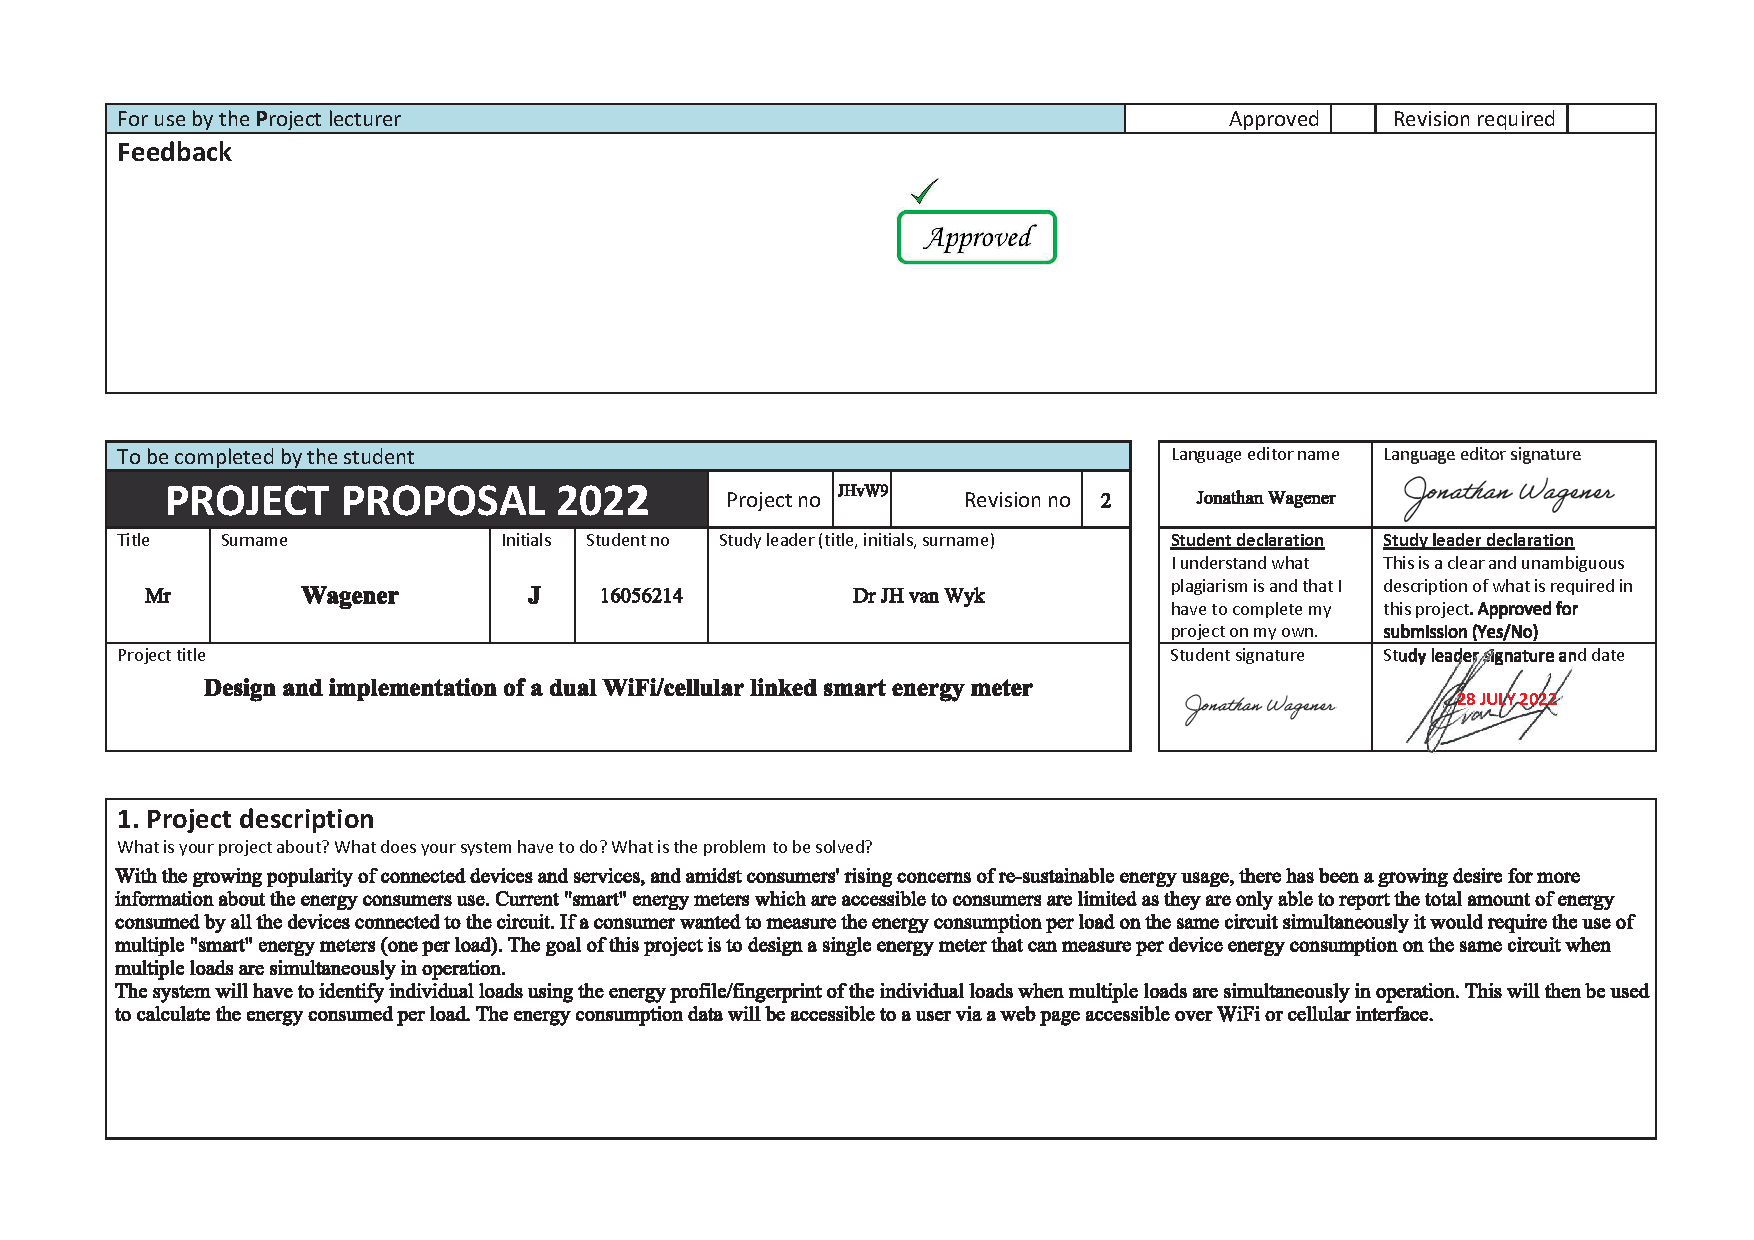
\includepdf[pages=-,landscape]{approved_proposal.pdf}

\addtocontents{toc}{\protect\contentsline{subsection}{1. Project description}{}\%}
\addtocontents{toc}{\protect\contentsline{subsection}{2. Technical challenges in this project}{}\%}
\addtocontents{toc}{\protect\contentsline{subsection}{3. Functional analysis}{}\%}
\addtocontents{toc}{\protect\contentsline{subsection}{4. System requirements and specifications}{}\%}
\addtocontents{toc}{\protect\contentsline{subsection}{5. Field conditions}{}\%}
\addtocontents{toc}{\protect\contentsline{subsection}{6. Student tasks}{}\%}

%% --- PART 3 ------------------------------------------------------------

\eprsec{Part 3. Main Report}
\newpage

%% Reset the page number style and count.
\pagenumbering{arabic}
\setcounter{page}{1}

%% Import the main report content
%%
%%  Department of Electrical, Electronic and Computer Engineering.
%%  EPR400/2 Final Report - Section 1.
%%  Copyright (C) 2011-2021 University of Pretoria.
%%

\section{Literature study}
An energy meter is a device used to measure the energy consumption of the active loads on a circuit. Most energy meters provide the total energy used, but do not provide per-load energy consumption. This information can be important to both consumers and energy providers.
 Consumers are able to better understand how they consume energy. The desired granularity of how the total energy is consumed is only achievable in three ways: first, the actual device can report on its own energy consumption; secondly, an energy meter may be installed for each device; and, finally, Non-Intrusive Load Monitoring (NILM) could be used.
\par
Energy providers are able to manage supply and demand more effectively which is necessary for the functionality of any energy grid \cite{Grid_predic}. Using modern prediction algorithms to analyse the granular information regarding how consumers use energy throughout the day can improve the accuracy of electric load forecasting (ELF), thus enabling energy providers to manage (and meet) the energy supply and demand more effectively \cite{7926112}.
\par
All electrical loads will produce a rising or falling edge when there is a change to their working state - this is indicated by the arrows pointing upwards or downwards in Figure~\ref{fig:1}. The state between the two transient edges is the steady state \cite{RN38}. Features that define a change to the working state can be defined as transient signatures and steady state signatures \cite{RN34}. In the 1980s, George Hart \cite{RN42} presented a method of load identification which allowed him to distinguish between multiple loads with one energy monitoring device. He pioneered the term Non-Intrusive Load Monitoring (NILM). Hart's method made use of the transients or (in his words) "step changes". 
\begin{figure}[H]
    \centering
    \includegraphics[width=0.8\textwidth]{Figures/Literature_study/Fig1.png}
    \caption{Examples of load signatures of household appliances as illustrated in \cite{RN42}.}
    \label{fig:1}
\end{figure}
As shown in Figure~\ref{fig:1}, Hart's method is only able to identify loads when a transition event that causes a significant change in the power draw is detected. The method's failure to make use of the steady state to identify loads reduces its effectiveness.
\par
Hart's original system was later improved in a number of ways. The first refinement resulted from innovation in data acquisition systems used for energy monitoring which has allowed for smaller changes in power to be measured at an increased sample rate. Most modern off-the-shelf energy monitoring systems make use of analogue-to-digital converters (ADCs) that have a resolution exceeding 10-bits \cite{RN48}. This is one of the most notable improvements. The increase in ADC resolution enables an energy monitor to measure a change in power exceeding \qty{11.23}{\watt}, with some energy monitors being able to measure a change as low as \qty{0.17}{\watt}. 
\par
Another improvement to the data acquisition systems was an increase in the sample rate - this has resulted in more harmonic information to identify unique loads \cite{RN52}. In order to distinguish between 20 - 40 loads, a sample rate of between 10 – 40 kHz is required \cite{RN52}. This allows for the identification of small power draw loads that would not have been detectable using Hart's original method.
\par
Saleh makes a case in favour of using specialised mathematical transforms for transient feature extraction - such as the Huang Hilbert Transform (HHT) with Ensemble Empirical Mode Decomposition (EEMD) (\cite{RN53}). While the author persuasively argues that this is an accurate and effective method of feature extraction, he does not expand much on the practical implementation of his method.
\par
The steady state can be disaggregated into many features that are unique to the particular state of a load. Some of the most common features include power variation, and time and current harmonics. These steady state features are currently being researched and tested \cite{8895360}.
One of the most notable features that has recently been studied is the V-I trajectory feature. 
\par
V-I trajectory allows for the clustering of similar load signatures in feature space. This is accomplished by projecting the instantaneous voltage and current signals to an XY-cartesian plane over one complete cycle. In Figure~\ref{fig:2}, some loads from the Controlled ON-OFF Loads Library (COOLL) are mapped in this way. The figure shows that every load's projection is distinct. 
\begin{figure}[H]
    \centering
    \includegraphics[width=0.5\textwidth]{Figures/Literature_study/VI_Projection.png}
    \caption{Examples of load projection from the COOLL data set as illustrated in \cite{8895360}.}
    \label{fig:2}
\end{figure}
Mulinari \emph{et al} integrated the features that came about as a result of the new feature extraction techniques into three existing detection algorithms (Ensemble, kNN and SVM) (\cite{8895360}). They recorded that the accuracy of the detection methods could vary from between \qty{70}{\%} and \qty{99.64}{\%} when identifying the loads contained in the COOLL dataset. The most significant result was that - even though all the features (existing and new) were combined by the detection algorithm - the accuracy of the prediction never fell below \qty{96.35}{\%}.     
\par
The detection methods used by Mulinari \emph{et al} (\cite{8895360}) are not the only algorithms that have been used in NILMs.
 Methods which use Hidden Markov models are still actively being researched. Two papers using Hidden Markov models were recently published in 2015 and 2018 \cite{RN38,RN40}. The Hidden Markov model (the original method used by Hart) uses statistical predictions to identify the current state of a load \cite{RN42}. As was the case in the original work of Hart, the results presented by Zhihao \emph{et al} \cite{RN38} and Jung \emph{et al} \cite{RN40} also only pertained to loads that caused significant power draw changes when a change in operation occurred. The research did not make any predictions or comment on the effectiveness of the device in a situation where it was used with loads which cause nominal power changes. 
 The effectiveness of the device is given in Bit-Error-Rate (BER). However, the authors do not provide any insight as to how to relate the BER to allow for a comparison to be drawn with the other methods discussed in the literature. The usefulness of these results as a benchmark against which other methods can be compared is therefore limited.
 \par
 The research of Zhihao \emph{et al}, \cite{RN38} and Jung \emph{et al}, \cite{RN40} was focused solely on theoretical application and only tested in simulations. Mubarok \emph{et al}, \cite{RN47} conducted similar research with the focus being on practical implementation. Their aim was to develop an algorithm that was simple to implement on an embedded processing platform. 
 Mubarok \emph{et al} implemented a method referred to as the radial basis function - this method is used to derive an unknown function from a set of inputs and known outputs. The authors use the FFT of the current signal as the input to the radial basis function. Once the function has been derived, it is implemented on the STM32F407VGT6 embedded platform. 
 The implemented radial basis function was able to identify the loads with an error margin of merely \qty{0.14}{\%} to \qty{4.84}{\%}. These results demonstrated that the practical radial basis function was able to detect loads accurately in most instances with an error rate that was commendably low. These findings were limited as the function needs to be trained for every possible combination comprised of the unique loads, and these combinations increase exponentially. In other words, if the number of unique loads was doubled, the resulting number of combinations would be 256. The radial basis function is an approximation function which uses a large number of linear matrix operations in order to make a prediction. Consequently, it has the disadvantage of being slowed down by the number of combinations due to the complexity cost being between $O(n^{2})$ and $O(n^{3})$ (with n being the number of samples).
 \par
A recent paper published in 2020 by Guohua \emph{et al} \cite{RN39} may provide a solution for this problem. They propose using a random forest algorithm - an algorithm which is commonly used to overcome classification and regression problems in a machine learning context. Unlike the radial basis function, the decision tree only makes use of a number of checks - no mathematical operations are performed when it makes its prediction. Here the complexity cost is $O(n log (n))$. This is substantially lower than that of the radial basis function.
Unfortunately, this method resulted in a slight decrease in accuracy. Using the same number of loads as Mubarok \emph{et al} as well as the large power loads used in \cite{8895360,RN38,RN40}, the resulting largest measured error margin was \qty{14}{\%} \cite{RN47}. 
As with the research done by Mubarok \emph{et al}, the use of a random forest algorithm in NILM has also only been simulated, its practical implementation not yet having been tested \cite{RN47}.
\par
Non-Intrusive Load Monitoring has seen significant improvement since Hart's original design in the 1980s \cite{RN42}. Most of these improvements and related innovations occurred within the last 10 years due to renewed interest in the field of energy consumption. There are two areas of focus where researchers improved the NILM design.
Firstly, the features used for identification and the detection methods used were improved upon. Mulinari \emph{et al} \cite{8895360} showed that by implementing new identification features into existing detection methods, the accuracy of these methods can be significantly improved. Furthermore, it was discovered that combining new features with new or improved detection methods also resulted in improved accuracy \cite{RN39,RN38,RN40,RN47}. 
Most of the newly developed algorithms' results were obtained via simulations and not through practical implementation, as previously mentioned. The exception to this was the work of Mubarok \emph{et al}, \cite{RN47}, who successfully implemented a NILM on an embedded platform. However, it was discussed that the method used was limited as the complexity and time needed to perform an identification increases exponentially with the number of loads.  
On the other hand, Guohua \emph{et al}, \cite{RN39} demonstrated that a NILM using a random forest algorithm can produce similar levels of accuracy as that of the method used by Mubarok \emph{et al} \cite{RN47}. The advantage of the random forest algorithm was that it needed significantly less time to compute, the time taken scaling with $O(nlog_{n})$ as opposed to $O(n^{2})$.
\par
Upon reviewing the relevant literature, it can be concluded that the work of Mubarok \emph{et al} \cite{RN47} (where the method's functionality was only demonstrated through simulations) may be improved upon by using the methods of Guohua \emph{et al} \cite{RN39} for practical implementation purposes. This can be done by implementing a decision tree on an embedded platform. It is proposed that these improvements will result in the accuracy of the prediction method increasing to \qty{95}{\%}. 

%% End of File.



%%
%%  Department of Electrical, Electronic and Computer Engineering.
%%  EPR400/2 Final Report - Section 2.
%%  Copyright (C) 2011-2021 University of Pretoria.
%%

\section{Approach}
The goal was to develop a smart energy meter to identify the real-time state of the connected loads. The energy meter was produced to meet a number of requirements -  systems and subsystems aimed at fulfilling each requirement respectively were combined to create a fully functioning end product.
\par
The point of departure for the design process was to split the energy meter into two distinct subsystems. The first was the analogue front end which facilitated a safe tie-in with the live 230V service. The energy meter and user was galvanically isolated from mains electricity supply. The second subsystem processed the sampled data, and created the interface through which the user can view and interact with this processed data.
\par 
The first part of the design (discussed in more detail in section 3, below) focused on the ADCs design requirements. 
An ADC and embedded platform were selected once the ENOB and sample rate were determined. The preferred outcome was to obtain an embedded system with an onboard ADC. However, such a platform which meets the design requirements was found to be unjustifiably expensive given its intended application. An alternative solution was thus to select the embedded platform and external ADC which still meets the design requirements but which would be more cost-effective.
\par
Once the ADC was selected, a circuit was built to galvanically isolate the device from mains electricity, to convert voltage, and to current signals to a range the ADC can measure.
Transformers (safety and current clamp), optocouplers and sense resistors were considered as potential isolation methods. The safety transformer was determined to be the most beneficial method with the least negligible drawbacks for voltage measurements. Meanwhile (as will be discussed in more detail later), the current clamp transformer was found as the best solution for the current measurement. Thereafter the complementary circuitry was designed to interface the transformer and current clamp to the respective ADCs.
\par
The completed analogue circuity was successfully simulated, after which the circuit schematics were transformed into hardware schematics. The hardware schematics were then used to create the physical circuity. Here a modular design was implemented to allow for individual sections of the circuit to be modified or changed if necessary as opposed to the entire circuit having to be re-designed or -constructed following possible change.
\par
The embedded platform and ADCs were interfaced with a serial communication protocol which allowed the two ADCs to sample the voltage and current simultaneously, reducing the need for phase compensation when calculating the power. The raw binary data that the ADC produced was converted to a floating point format, and calibrated to reflect the actual values of the voltage and current.\footnote[1]{Implemented on embedded platform} 
\par
Two digital FIR filters - an Anti-aliasing and a \qty{50}{\hertz}~low-pass filter - were designed from first principles and then applied to the raw signal sampled by the ADCs. These filters used different window functions to fulfil different functions. The Anti-aliasing filter was used to prevent the occurring of unwanted spectral components in the frequency system of interest as a result of the sampling process. The \qty{50}{\hertz}~low-pass filter was designed to isolate the \qty{50}{\hertz} power component from the harmonics to make the power measurements more accurate.\footnotemark[1]
\par
Thereafter, a data collection program was developed to collect the necessary features for the identification of loads. These features included the real and reactive power components, as well as the harmonics of the current load which were produced by performing the FFT transform on the current signal.
\par 
A detection algorithm was then developed, the main goal being to obtain an algorithm which offered sufficient accuracy with the lowest possible performance overhead. A number of method algorithm options were considered, namely classification decision trees, neural networks and K-Nearest Neighbors. The investigation found that multiple decision tree classifiers for the creation of a random forest was the method which best fulfilled the necessary requirements. As such, the collected data was used to train the decision trees and create the forest.\footnote[2]{Implemented on personal computer}
\par
The hardware and software were then combined. The figure~\ref{fig:Flow_1} depicts the final interfacing of the main program, which called all the above software, resulting in a completed system that performed the energy calculation and load detection. The main program then presented the data on a web page for the user to view in accordance with the flowchart depicted in figure~\ref{fig:Flow_1}

\begin{figure}[H]
    \centering
    \includegraphics[width=0.7\textwidth]{Figures/Flow/FLow_1.png}
    \caption{Flow chart of software functions integrated into a complete detection system.}
    \label{fig:Flow_1}
\end{figure}


 
\newpage

%% End of File.


%%
%%  Department of Electrical, Electronic and Computer Engineering.
%%  EPR400/2 Final Report - Section 3.
%%  Copyright (C) 2011-2021 University of Pretoria.
%%

\section{Design and implementation}

\subsection{Design summary}
% Please add the following required packages to your document preamble:
% \usepackage{graphicx}
\begin{table}[H]
\resizebox{\textwidth}{!}{%
\begin{tabular}{|l|l|l|}
\hline
\textbf{Deliverable or task} &
  \textbf{Implementation} &
  \textbf{\begin{tabular}[c]{@{}l@{}}Completion of deliverable\\ or task, and section in the \\ report\end{tabular}} \\ \hline
\begin{tabular}[c]{@{}l@{}}Design of mains voltage interface\\ and attenuation circuit \end{tabular} & \begin{tabular}[c]{@{}l@{}}The student completed the design\\ from first principles\end{tabular} & \begin{tabular}[c]{@{}l@{}}Complete\\ Section~\ref{sec:D_V}\end{tabular} \\ \hline

\begin{tabular}[c]{@{}l@{}}Design of mains current interface\\ and attenuation circuit \end{tabular} & \begin{tabular}[c]{@{}l@{}}The student completed the design\\ from first principles\end{tabular} & \begin{tabular}[c]{@{}l@{}}Complete\\ Section~\ref{sec:D_I}\end{tabular} \\ \hline

\begin{tabular}[c]{@{}l@{}}Design of differential ADC input driver\end{tabular}                      & \begin{tabular}[c]{@{}l@{}}The student completed the design\\ from first principles\end{tabular} &
\begin{tabular}[c]{@{}l@{}}Complete\\ Section~\ref{sec:D_ADC}\end{tabular} \\ \hline

\begin{tabular}[c]{@{}l@{}}Design of \qty{\pm 2.5}{\volt} reference \end{tabular}                    & \begin{tabular}[c]{@{}l@{}}The student completed the design\\ from first principles\end{tabular} &
\begin{tabular}[c]{@{}l@{}}Complete\\ Section~\ref{sec:D_ref}\end{tabular} \\ \hline

\begin{tabular}[c]{@{}l@{}}Hardware design and  \\ implementation voltage interface \end{tabular}    & \begin{tabular}[c]{@{}l@{}l@{}}The student implemented \\ the hardware  design  on \\ veroboard from first principles \end{tabular} &
\begin{tabular}[c]{@{}l@{}}Complete\\ Section~\ref{sec:H_V}\end{tabular} \\ \hline

\begin{tabular}[c]{@{}l@{}}Hardware design and   \\ implementation current interface \end{tabular}   & \begin{tabular}[c]{@{}l@{}l@{}}The student implemented \\ the hardware  design  on \\ veroboard from first principles\end{tabular} &
\begin{tabular}[c]{@{}l@{}}Complete\\ Section~\ref{sec:H_I}\end{tabular} \\ \hline

\begin{tabular}[c]{@{}l@{}}Hardware design and   \\implementation ADC input driver\end{tabular}      & \begin{tabular}[c]{@{}l@{}l@{}}The student implemented \\ the hardware  design  on \\ veroboard from first principles\end{tabular} & 
\begin{tabular}[c]{@{}l@{}}Complete\\ Section~\ref{sec:H_ADC}\end{tabular} \\ \hline

\begin{tabular}[c]{@{}l@{}}Hardware design and \\implementation \qty{\pm 2.5}{\volt} reference \end{tabular} & \begin{tabular}[c]{@{}l@{}l@{}}The student implemented \\ the hardware  design  on \\ veroboard from first principles\end{tabular} & 
\begin{tabular}[c]{@{}l@{}}Complete\\ Section~\ref{sec:H_V_Ref}\end{tabular} \\ \hline

\begin{tabular}[c]{@{}l@{}}PRU ADC Interface Software\end{tabular}  & \begin{tabular}[c]{@{}l@{}l@{}}The student implemented a custom version of \\ the SPI protocol from first principles to \\ interface the ADC and PRU  \end{tabular} &
\begin{tabular}[c]{@{}l@{}}Complete\\ Section~\ref{sec:PRU}~and~\ref{sec:Sample} \end{tabular} \\ \hline

\begin{tabular}[c]{@{}l@{}}Digital FIR Filter Design\end{tabular}  & \begin{tabular}[c]{@{}l@{}l@{}}The student designed the filter from first principles \\ The implementation was done using a library \end{tabular} & 
\begin{tabular}[c]{@{}l@{}}Complete\\ Section~\ref{sec:Filter}\end{tabular} \\ \hline

\begin{tabular}[c]{@{}l@{}}Development of the data collection\\ system\end{tabular}  & \begin{tabular}[c]{@{}l@{}l@{}l@{}}The student designed and implemented a custom \\ automated data collection system from first principles.\\The GUI used to control the system \\ was implemented using a library\end{tabular} &
\begin{tabular}[c]{@{}l@{}}Complete\\ Section~\ref{sec:DC}\end{tabular} \\ \hline

\begin{tabular}[c]{@{}l@{}}Development of the decision tree \end{tabular}  & \begin{tabular}[c]{@{}l@{}l@{}}The student implemented a custom version of \\ the SPI protocol from first principles to \\ interface the ADC and PRU  \end{tabular} &
\begin{tabular}[c]{@{}l@{}}Complete\\ Section~\ref{sec:DT}\end{tabular} \\ \hline

\begin{tabular}[c]{@{}l@{}}Training of the decision tree \\ and creation of the forest \end{tabular} & \begin{tabular}[c]{@{}l@{}l@{}l@{}l@{}}The student implemented a decision tree \\algorithm from first principles with the particular \\ implementation of the decision \\ tree forest being completely original \end{tabular} &
\begin{tabular}[c]{@{}l@{}}Complete\\ Section~\ref{sec:deply_DT}\end{tabular} \\ \hline

\begin{tabular}[c]{@{}l@{}}Full system integration \\ GUI development \end{tabular} & \begin{tabular}[c]{@{}l@{}l@{}l@{}l@{}l@{}l@{}} The system was fully integrated as a Dash Application.\\The GUI components provided by Dash are taken off the self. \\ All the functions that generate the information \\that GUI displays are designed and \\integrated using first principles\end{tabular} &
\begin{tabular}[c]{@{}l@{}}Complete\\ Section~\ref{sec:Full}\end{tabular} \\ \hline

\end{tabular}%
}
\caption{Design summary.}
\label{tab:Design_summary}
\end{table}
\newpage
\subsection{Theoretical analysis}

\subsubsection{ADC Sample rate and resolution requirements}
\label{sec:D_V}
All ADCs have three main specifications: the voltage range they can measure, the number of bits they can use (resolution) to represent that voltage, and the speed (sample rate) at which the conversion takes place. The accuracy of the measurement is affected by all three these specifications. 
The effective number of bits (ENOB) is the measure of how much resolution an ADC will have in a particular system, this being dependant on all three of the above specifications. Increasing the ENOB measure also increases accuracy and allows smaller signals to be measured. However, this increase comes at a trade off for every bit increase to ENOB. The design complexity increases exponentially. 
\par
The following calculations were used to determine the minimum ENOB required for the voltage signal. The specification for household voltage supplied in South Africa is \qty{\pm 230}{\volt} \qty{\pm 10}{\percent}, meaning that the range over which the samples needed to be taken can be calculated by equations\ref{eq:1}~and~\ref{eq:2}
\begin{equation}
\label{eq:1}
\begin{split}
    V_{min} &= 230 \;V \times (100-10 \%) \;\;\\
            &= 230 \;V \times (90 \%) \;\;\\
            &= 207 \; V \; ,
\end{split}
\end{equation}
\begin{equation}
\label{eq:2}
\begin{split}
    V_{max} &= 230 \;V \times (100+10 \%) \;\;\\
            &= 230 \;V \times (110 \%) \;\;\\
            &= 253 \; V \; .
\end{split}
\end{equation}
The root-mean-square (RMS) Voltage was used to calculate the values above. The definition of effective or RMS value that was provided in \cite{alexander_o._2021} is that the effective value of a periodic current is the DC current that delivers the same average power to a resistor as the periodic current. Using the RMS value would result in a design that cannot measure the AC voltage waveform over the desired range as this is not the peak-to-peak voltage of the signal. The actual peak-to-peak values of the voltage signal were derived using the equations presented below:
    \begin{equation}
    \label{eq:3}
    \begin{split}
    V(max)_{pk-pk} &= [V_{max} - (V_{min})] \times \sqrt{2} \;\;\\
              &= [253 \; V - (-253 \; V)] \times \sqrt{2} \;\;\\
              &= 715,59 \; V \; ,
    \end{split}
    \end{equation}

    \begin{equation}
    \label{eq:4}
    \begin{split}
    V(min)_{pk-pk} &= [V_{max} - (V_{min})] \times \sqrt{2} \;\;\\
              &= [207 \; V - (-207 \; V)] \times \sqrt{2} \;\;\\
              &= 585.48 \; V \; .
    \end{split}
    \end{equation}
Figure~\ref{fig:Volt_sim} is a mathematical simulation of a \qty{50}{\hertz} sine wave with the largest possible amplitude the system was expected to measure. Indicated in the figure are the $V_{rms}$ and $V_{max}$ values - the $V_{max}$ value is noticeably larger than $V_{rms}$ value.
\begin{figure}[H]
    \centering
    \includegraphics[width=0.7\textwidth]{Figures/RMS/Vrms.png}
    \caption{Mathematical simulation of expected voltage signal.}
    \label{fig:Volt_sim}
\end{figure}
A design error of \qty{1.0}{\percent} was chosen for the voltage measurement in order to prevent the desired error of the power measurement from exceeding \qty{\pm 2.5}{\percent}. This allows for a \qty{\pm 1.5}{\percent} error in the rest of the system. Equation~\ref{eq:5} below was used to convert the \qty{1.0}{\percent} error to a voltage value in relation to the smallest expected peak-to-peak voltage signal 
\begin{equation}
\label{eq:5}
\begin{split}
    \Delta V &= 1\% \times V(min)_{pk-pk} \; V \\
             &= 1\% \times  585.48\; V \\
             &= 5.85 \; V .
\end{split}
\end{equation}

Using the result from equation~\ref{eq:5}, the number of quantisation levels required to express the maximum peak-to-peak voltage while maintaining the design error was calculated using equation~\ref{eq:6},
\begin{equation}
\label{eq:6}
\begin{split}
    Levels  &= \frac{V(max)_{pk-pk}}{\Delta V} \\
            &= \frac{715.59}{5.85} \\
            &= 122.22\\
            &\approx 123.
\end{split}
\end{equation}
Using the number of quantisation levels from equation~\ref{eq:6} , the minimum ENOB were obtained using equation~\ref{eq:7},
\begin{equation}
\label{eq:7}
\begin{split}
    ENOB    &= log_{2}(Levels) \\
            &= log_{2}(123) \\
            &= 6.93\\
            &\approx 7\; bits.
\end{split}
\end{equation}
Therefore, only a 7-bit ADC is required to sample the voltage signal while maintaining an error of less than \qty{\pm 1.0}{\percent}.
\par
A similar process was followed to calculate the ENOB required to represent the current signal as the process used for sampling the voltage signal. The load's current draw is dependant on its voltage and power rating. This means that both the voltage and power draw values must be accounted for when calculating the range of current values needing to be measured.
\par
Equation~\ref{eq:8} and equation~\ref{eq:9} are used to calculate the minimum and maximum current values that the system is expected to be able to measure,
\begin{equation}
\label{eq:8}
\begin{split}
    P_{min_{rms}}                   &= V_{max_{rms}} \cdot I_{min_{rms}} \\
    2 \; W \;                       &= 253 \; V \; \cdot I_{min_{rms}} \\
    \therefore \; I_{min_{rms}}     &= \frac{2 \; W \;}{253 \; V} \\
                                    &= 7.9051 \; mA \; ,\\
\end{split}
\end{equation}

\begin{equation}
\label{eq:9}
\begin{split}
    P_{max_{rms}}                   &= V_{min_{rms}} \cdot I_{max_{rms}} \\
    8000 \; W \;                    &= 207 \; V \; \cdot I_{max_{rms}} \\
    \therefore \; I_{max_{rms}}     &= \frac{8000 \; W \;}{207 \; V} \\
                                    &= 38.647 \; A.\\
\end{split}
\end{equation}


The Figure~\ref{fig:Current_Sim} depicts two current signals. The left Figure~\ref{fig:Current_Sim_a} is the smallest possible signal that the system is expected to measure. The right Figure~\ref{fig:Current_Sim_b} is the largest possible signal that the system is expected to measure.

\begin{figure}[H]
     \centering
     \begin{subfigure}[b]{0.495\textwidth}
        \centering
        \includegraphics[width=1.0\textwidth]{Figures/RMS/Irms_min.png}
        \caption{The smallest current signal.}
        \label{fig:Current_Sim_a}
     \end{subfigure}
     \hfill
     \begin{subfigure}[b]{0.495\textwidth}
        \centering
        \includegraphics[width=1.0\textwidth]{Figures/RMS/Irms_max.png}
        \caption{The largest current signal.}
        \label{fig:Current_Sim_b}
     \end{subfigure}
        \caption{The smallest and largest current signals that are expected to be measured.}
        \label{fig:Current_Sim}
\end{figure}

The data in Figure~\ref{fig:Current_Sim_a} shows that the smallest possible current value is \qty{11.18}{\mA}. The largest possible value is \qty{54.656}{\ampere}. However, unlike the voltage, this accuracy value only applies to loads that draw over \qty{1.2}{\ampere}. Thus, in order to maintain a measurement error of less than \qty{\pm 2.5}{\percent}, a design error of \qty{\pm 1.0}{\percent} is expected - the value of which is calculated by equation~\ref{eq:10},

\begin{equation}
\label{eq:10}
\begin{split}
    \Delta I &= 1\% \times 1.2 \times \sqrt{2} \; A\\
             &= 1\% \times  3.39\; A \\
             &= 33.94 \; mA .
\end{split}
\end{equation}

Since the above calculated value of \qty{33.94}{\mA} is larger than \qty{11.18}{\mA} calculated in equation~\ref{eq:11} above, the ENOB can be calculated, as in

\begin{equation}
\label{eq:11}
\begin{split}
    Levels  &= \frac{I(max)_{pk-pk}}{I(min)} \\
            &= \frac{109.31}{11.18 \; mA} \\
            &= 9777.28\\
            &\approx 9778.
\end{split}
\end{equation}

Using the number of levels calculated by equation~\ref{eq:11} above, this can then be expressed as ENOB using equation~\ref{eq:12},
\begin{equation}
\label{eq:12}
\begin{split}
    ENOB    &= log_{2}(Levels) \\
            &= log_{2}(9778) \\
            &= 13.26\\
            &\approx 14\; bits.
\end{split}
\end{equation}

Comparing the results from equations~\ref{eq:7}~and~\ref{eq:12}, it is clear that an ADC which matches or exceeds 14 bits is required. As most ADCs do not come with a resolution of 14 bits, a 16-bit ADC is selected.
\par
The sample rate of the ADC was selected to exceed that of \qty{49}{\kHz}. This is because the main features required for detecting loads are the harmonics a device will create while in operation. The harmonics will be calculated using an FFT transform on the current signal. Only the odd harmonics are used. With a sample rate of \qty{49}{\kHz}, this implies that the FFT transform will have a frequency range of
\qty{24.5}{\kHz}. Since only the odd harmonics are used for load identification, a total of 245 harmonics can be used to fingerprint loads. Following the above criteria, the MCP33131D-10 from Microchip was selected based on the specifications summarised in Table~\ref{tab:ADC_Summary} below: 
\begin{table}[H]
\small
\centering
\begin{tabular}{|ccc|}
\hline
\multicolumn{3}{|c|}{MCP33131D-10}                 \\ \hline
\multicolumn{1}{|c|}{Parameter}                     & \multicolumn{1}{c|}{Minimum requirement}  & Actual                            \\ \hline
\multicolumn{1}{|c|}{Sample Rate}                   & \multicolumn{1}{c|}{\qty{ \pm 49}{\kHz}}  & \qty{\pm 1}{\MHz}                 \\ \hline
\multicolumn{1}{|c|}{Resolution}                    & \multicolumn{1}{c|}{14-bits}              & 16-bits                           \\ \hline
\multicolumn{1}{|c|}{Input Range}   & \multicolumn{1}{c|}{\qty{\pm 5.0}{\volt}}                 & \qty{\pm 5.1}{\volt}              \\ \hline
\end{tabular}%
\caption{Summary of the ADC specifications that are required to meet the needs of the application \cite{Microchip:MCP33131D}.
}
\label{tab:ADC_Summary}
\end{table}
Since the ADC is a precision 16-bit ADC, it requires an external voltage reference that maintains the same level of accuracy. Therefore, the MAX6250 (a precision \qty{5.0}{\volt}) was selected as the external voltage reference. This is because the voltage reference has a very low noise level of \qty{\pm 1.5}{\uV} peak-to-peak - this being far below the ADC's quantisation error.

\subsubsection{Mains Voltage Signal Isolation and Interface}
\label{sec:Mains_Voltage_Signal_Isolation_and_Interface}
There are many known methods for measuring a live voltage signal using a microcontroller. These include using a shunt resistor in series to create a voltage drop that is low enough for the ADC to measure. However, it offers little to no protection for the device and the user. One way of mitigating this is to create a voltage drop using multiple resistors in series. Implementing this design can isolate the device and user in the event that a resistor fails.
However, this is still not a perfect solution as it results in the addition of multiple points of failure.
\par
There are two methods which may be used to mitigate this potential danger by completely isolating the system from the potentially dangerous live voltage supply. 
The first method uses an optocoupler to completely isolate the live supply from the device performing the voltage measurement. The device makes use of a LED with a brightness output which is proportional to the supplied voltage. A photodiode is then used to convert this light to a voltage signal, the signal being dependent on the brightness of the LED. One of advantage of this method is that there is no interference with the actual voltage supply. However, the disadvantage is that there is no linear output proportional to the voltage input, there thus needing to be a calibration step in software or hardware to produce this linear output.
\par
The Figure~\ref{fig:V_interface} below shows a second alternative method via which to isolate and step down the dangerous voltage level using a safety transformer. 
\begin{figure}[H]

  \begin{center}
    \begin{circuitikz}
        \ctikzset{resistors/scale=0.7, capacitors/scale=0.6}
        \draw (0,0) -- ++(0,4) node[above](Live){$Neutral$} ++(0,0) ++(0,-1) to[short, *-] (2,3)
        (2,0) -- ++(0,4) node[above](Neutral){$Live$} ++(0,0) ++(0,-1)
        (2,3) node[transformer, circuitikz/inductors/coils=7,anchor=A1](T){}
        (T.A2) to[short, -*] (T.A2)
        (T.B2) node[ground](GND){} ++(0,-1) 
        (T.B1) to [R=$R_1$] ++(2,0) -- ++(0.5,0)
        node[op amp, anchor=-](OA1){\texttt{OA1}}
        (OA1.-) ++(-0.5,0) -- ++(0,1.5) -- ++(0.5,0)
        to[R=$R_2$] ++(2,0) coordinate(FB) 
        (OA1.out) |- (FB)
        (OA1.out) -- ++(1,0) node [right] {$V_{out}$}
        (OA1.+) -| ++(-0.5,-1.1) node[ground](GND){} ++(0,0)
      ;
    \end{circuitikz}
    \caption{Voltage interface circuit.}
    \label{fig:V_interface}
  \end{center}
\end{figure}
 The safety transformer depicted in the circuit above is rated to transform a \qty{230}{\volt} down to \qty{12}{\volt}. As such, the max peak-to-peak voltage is \qty{37.34}{\volt}. Since the voltage is still too high for the specified ADC(MCP33131D-10) even after implementing the safety transformer, the voltage must be transformed to a range of \qty{\pm 2.5}{\volt}. This transformation is affected using a voltage amplifier comprised of an operational amplifier and two resistors, the amplification factor being governed by equation~\ref{eq:13}
\begin{equation}
\label{eq:13}
    V_{out} = V_{in} \cdot \frac{R_{2}}{R_{1}} \;, 
\end{equation}
respectfully \cite{design_with}.

Substituting $V_{in} =$\qty{37.34}{\volt}, $V_{out} =$ \qty{2.5}{\volt} and selecting a value of \qty{10}{\kohm} for $R_{1}$, results in a value of \qty{1250}{\ohm} for $R_{2}$.

\subsubsection{Mains Current Signal Isolation and Interface}
\label{sec:D_I}
As mentioned in the section above, there are many ways in which to sample a live \qty{230}{\volt} current signal. One method is to insert a shunt resistor between the current supply and the load on the live voltage wire. By measuring the voltage over the shunt resistor (which has a precise resistance value that is known), the current flowing to the load can be calculated using ohms law. However, this method has the potential to place the device and its user in danger should the resistor fail.
\par
A safer solution is to use a current clamp, a transformer which typically has a split core and can wrap around the live wire. A current is produced through the wire by placing the core around it. This current can then be converted into a voltage using a resistor. However, not all current clamps are necessarily equally suited to perform this function. Current clamps can vary in three distinct ways:
\begin{itemize}
    \item First, the number of windings between the primary coil and the secondary coil may vary. This number is directly responsible for the range of currents which the transformer is rated to measure at its specified accuracy level. 
    \item Secondly, the magnitude of the burden resistor may differ, this having a direct impact on the linear region and accuracy of the current signal produced by the transformer. 
    \item Finally, the accuracy class of the current clamps may vary - this accuracy being determined by the maximum rated error that occurs in the linear measurement region of the current clamp.
\end{itemize}

Having taken all of the above factors as well as the desired accuracy specified in the design requirements into account, the ATO-75-B1I-D10 current clamp from LEM was selected as most suitable for the design. The Table~\ref{tab:CC_Summary} below is a summary of requirements that the ATO-75-B1I-D10 met or exceeded resulting in it being selected as most suitable for this particular application.

\begin{table}[H]
\small
\centering
\begin{tabular}{|ccc|}
\hline
\multicolumn{3}{|c|}{ATO-75-B1I-D10 with $R_{br} = $ \qty{4}{\ohm}}                 \\ \hline
\multicolumn{1}{|c|}{Parameter} & \multicolumn{1}{c|}{Minimum requirement} & Actual \\ \hline
\multicolumn{1}{|c|}{Primary current ($I_{p}$)}           & \multicolumn{1}{c|}{\qty{ \pm 75}{\ampere}}  & \qty{\pm 125}{\ampere}                              \\ \hline
\multicolumn{1}{|c|}{Rated primary current ($I_{pr}$)}    & \multicolumn{1}{c|}{\qty{ \pm 75}{\ampere}}  & \qty{\pm 75}{\ampere}                               \\ \hline
\multicolumn{1}{|c|}{Frequency bandwidth (\qty{-3}{\dB})} & \multicolumn{1}{c|}{\qty{49}{\kHz}}          & \qty{500}{\kHz}                                     \\ \hline
\multicolumn{1}{|c|}{Ratio error ($\varepsilon$)}         & \multicolumn{1}{c|}{\qty{\pm 2}{\percent}}   & \qty{\pm 1.0}{\percent}                             \\ \hline
\multicolumn{1}{|c|}{Linearity error ($\varepsilon_{L}$)}  & \multicolumn{1}{c|}{\qty{\pm 0.5}{\percent}} & \qty{\pm 0.1}{\percent}                             \\ \hline
\multicolumn{1}{|c|}{Rated secondary Current ($I_{sr}$)}  & \multicolumn{1}{c|}{NA}                      & \qty{\pm 75}{\mA}                                   \\ \hline
\multicolumn{1}{|c|}{Rated transformation ratio ($K_{ra}$)}          & \multicolumn{1}{c|}{NA}                      & \qty[per-mode = symbol]{1000}{\ampere \per \ampere} \\ \hline
\end{tabular}%
\caption{Summary of the specifications that are required to meet the needs of the application \cite{LEM:ATO-75-B1I-D10}.
}
\label{tab:CC_Summary}
\end{table}

 
The circuit diagram in Figure~\ref{fig:I_interface} below depicts the current clamp and the burden resistor which create a voltage signal proportional to the current flowing through the live supply wire.

\begin{figure}[H]
  \begin{center}
    \begin{circuitikz}
        \ctikzset{resistors/scale=0.7, capacitors/scale=0.6}
        \draw (0,0) -- ++(0,4) node[above](Live){$Neutral$} ++(0,0)
        (2,0) -- ++(0,4) node[above](Neutral){$Live$} ++(0,0) ++(0,-1)
        to[iloop2, name=I] ++(0,-2)
        (I.i-) |- ++(1,-2) coordinate(R) 
        (I.i+) ++(1,0) to [R=$R_{br}$] (R)
        (R) ++(-0.5,0) node[ground](GND){} ++(0,-0.5)
        (I.i+) -- ++(1.5,0)
        node[op amp, anchor=+](OA1){\texttt{OA1}}
        (OA1.-) |- ++(3,1) |- (OA1.out) -- ++(1,0) 
        to [R=$R_1$] ++(2,0) -- ++(1.0,0)
        node[op amp, anchor=-](OA2){\texttt{OA2}}
        (OA2.-) ++(-0.5,0) -- ++(0,1.5) -- ++(0.5,0)
        to[R=$R_2$] ++(2,0) coordinate(FB) 
        (OA2.out) |- (FB)
        (OA2.out) -- ++(1,0) node [right] {$V_{out}$}
        (OA2.+) -| ++(-0.5,-1.1) node[ground](GND){} ++(0,0);
    \end{circuitikz}
    \caption{Current interface circuit.}
    \label{fig:I_interface}
  \end{center}
\end{figure}
With the burden resistor $R_{br} = $ \qty{4}{\ohm}, the ATO-75-B1I-D10 current clamp indicated in the circuit schematic presented in Figure~\ref{fig:I_interface} is rated to achieve the error values stated in Table~\ref{tab:CC_Summary} above. This resistor is nominal compared to the others used in the circuit. As such, the voltage signal produced over $R_{br}$ is susceptible to loading, which could make the amplification of the signal all but impossible. 
A buffer amplifier was placed between the burden resistor and the amplification circuit in order to mitigate the loading of the signal. The signal is then amplified using a voltage amplifier comprised of an operational amplifier and two resistors, with the amplification factor being governed by the equation~\ref{eq:14}
\begin{equation}
\label{eq:14}
    V_{out} = V_{in} \cdot \frac{R_{2}}{R_{1}} , 
\end{equation}
respectfully \cite{design_with}.
Where $V_{in}$ is defined by equation~\ref{eq:15}
\begin{equation}
\label{eq:15}
    V_{in_{max}} = I_{sr} \cdot 4 \Omega \;. 
\end{equation}
Substituting $I_{sr} =$\qty{106.07}{\mA} into equation~\ref{eq:15} above yields, $V_{in_{max}} =$ \qty{424.26}{\mV}.With $V_{out_{max}} = \frac{V_{ref}}{2} =$~\qty{2.5}{\volt}. Selecting a value of \qty{32}{\ohm} for $R_{1}$, results in a value of \qty{826}{\ohm} for $R_{2}$.

\subsubsection{Differential ADC input driver}
\label{sec:D_ADC}
The differential ADC works by sampling the difference between two signals. Thus, the original signal needs to be converted to a differential signal in order to make use of the full 16-bit range of the MCP33131D-10 ADC. It is imperative to note that, while the data sheet of the MCP33131D-10 states that it can measure $\pm {V_{ref}}$, this specification is somewhat ambiguous and potentially misleading. The specification actually refers to the difference between the "positive" and "negative" inputs to the ADC - not to the inputs themselves. The ADC is also only designed to have a positive voltage applied to both inputs. Thus, the original signal needs to be modified  to use the ADC's entire range. 
\par
The before-mentioned modification was done by designing a differential ADC driver (depicted in Figure~\ref{fig:ADC_Driver}) to modify the signal. The purpose of the differential ADC driver is to take a signal and apply $-\frac{V_{ref}}{2}$ offset - after which the modified signal is then inverted using an inverting unity gain amplifier. Offsets are applied to ensure that the signal is positive and in the expected range for the ADC. An offset of $\frac{V_{ref}}{2}$ is thus also applied to the original signal using a normal unity gain amplifier. 
\begin{figure}[H]
  \begin{center}
    \begin{circuitikz}
        \ctikzset{resistors/scale=0.7, capacitors/scale=0.6}
        \draw (0,0) ++(0,2) node[left](V_25){$+2.5\;V$} ++(0,0) -- ++(1,0)
        to [R=$R_1$] ++(2,0) ++(0,-0.5) -- ++(2,0)
        node[op amp, anchor=-](OA1){\texttt{OA1}}
        (OA1.+) -| ++(-0.5,-0.5) node[ground](GND){} ++(0,0)
        (OA1.-) ++(-0.5,0) -- ++(0,1.5) -- ++(0.5,0)
        to[R=$R_5$] ++(2,0) coordinate(FB) 
        (OA1.out) |- (FB)
        (OA1.out) -- ++(1,0)
        node[op amp, anchor=+](OA2){\texttt{OA2}}
        (OA2.out) -| ++(0,1.5) -| (OA2.-)
        (OA2.out) to[R=$R_8$] ++(1.2,0) -- ++(0.7,0) node[right](V_+){$V-_{out}$} ++(0,0) 
        ++(-0.7,0) -- ++(0,-0.2) to[C=$C_1$] ++(0,-0.8)
        node[ground](GND){} ++(0,0)

        (0,0) node[left](V_in){$V_{in}$} ++(0,0) -- ++(1,0)
        -| ++(0,1) to [R=$R_2$] ++(2,0) -- ++(0,1)
        
        (0,0) -- ++(1,0)
        -| ++(0,-1) to [R=$R_3$] ++(2,0) -- ++(0,-1)
        
        (0,0) ++(0,-2) node[left](V_25){$-2.5\;V$} ++(0,0) -- ++(+1,0)
        to [R=$R_4$] ++(+2,0) ++(0,+0.5) -- ++(2,0)
        node[op amp, noinv input up, anchor=+](OA3){\texttt{OA3}}
        (OA3.-) -- ++(-0.5,0) -- ++(0,-1) coordinate(FB) 
        (FB) -- ++(0,-0.25) to [R=$R_6$] ++(0,-1.2)
        to node[ground](GND){} ++(0,0)
        (OA3.out) -- ++(0,-1.5)
        to [R=$R_7$] (FB)
        (OA3.out) -- ++(1,0)
        node[op amp, anchor=+](OA4){\texttt{OA4}}
        (OA4.out) -| ++(0,1.5) -| (OA4.-)
        (OA4.out) to[R=$R_9$] ++(1.2,0) -- ++(0.7,0) node[right](V_+){$V+_{out}$} ++(0,0) 
         ++(-0.7,0) -- ++(0,-0.2) to[C=$C_2$] ++(0,-0.8)
        node[ground](GND){} ++(0,0)
        ;
    \end{circuitikz}
    \caption{Differential ADC input driver.}
    \label{fig:ADC_Driver}
  \end{center}
\end{figure}
The Figure~\ref{fig:ADC_Driver} above depicts a circuit schematic that was designed. The non-inverting unity gain amplifier is comprised of an operational amplifier (OA1) and resistors $R_{1}$,$R_{2}$ and $R_{3}$. The inverting unity gain amplifier is comprised of an operational amplifier (OA2) and resistors $R_{4}$,$R_{5}$ and $R_{6}$. Since this ADC driver is comprised of unity gain amplifiers thus the resistors $R_{1}$ through  $R_{6}$ are all ideally the same value of \qty{10}{\kohm}. The differential signals are then buffered by the operational amplifiers (OA3 and OA4) to prevent loading. This signal is then run though a passive first order anti aliasing RC filter who's cut off frequency is defined by the following equation~\ref{eq:16}
\begin{equation}
    f_{c}   = \frac{1}{2 \pi R C},
    \label{eq:16}
\end{equation}
respectfully \cite{design_with}.
With a  desired cutoff frequency of \qty{20}{\kHz} the \qty{2.2}{\nF} capacitors  were specified $C_{1}$ and $C_{2}$. The resistors $R_{8}$ and $R_{9}$ were then calculated to have a value of  \qty{3617}{\ohm} using equation~\ref{eq:16}. Since \qty{3617}{\ohm} is not a standard resistor value a resistor value of  \qty{3300}{\ohm} was selected. Equation~\ref{eq:16} was then use again to calculate the as design new cut off frequency of \qty{21.9}{\kHz}. 


\subsubsection{Voltage Reference}
\label{sec:D_ref}
The Figure~\ref{fig:ADC_Driver} depicted above is the differential ADC driver. On the left, the design requires both a positive and negative \qty{\pm 2.5}{\volt} references to offset the signals. Since this design is used for both voltage and current signals, two of each reference are required.
\par
In order to create these four references, buffers are used instead of creating a duplicate of the left side of the circuit depicted below in Figure~\ref{fig:Vref_circuit}.

\begin{figure}[H]
  \begin{center}
    \begin{circuitikz}
        \ctikzset{resistors/scale=0.7, capacitors/scale=0.6,diodes/scale=0.6}
        \draw (0,0) node[ground](GND){} ++(0,0)
        to [zzD*, l=$LM385Z$] ++(0,6)
        to [R=$R_{s}$] ++ (0,2)
        node[vcc](vcc){$9V$} ++(0,0)
        (0,0) -- ++(2,0) 
        node[op amp,noinv input up, anchor=-](OA1){\texttt{OA1}}
        (OA1.+) -| ++(-0.5,1) coordinate(C1)
        to [R=$R_{1}$] ++(0,3.5) coordinate(C2)
        (OA1.out) -| ++(0,1.5) coordinate(C3) 
        (C1) to [R=$R_{2}$] (C3)
        (C2) -- ++(-1.5,0)
        (C2) -- ++(3.88,0) coordinate(C4)
        (OA1.out) -- ++(1,0) coordinate(C5)
        
        
        (C4) -- ++(0,1.2)
        node[op amp, anchor=+](OA2){\texttt{OA2}}
        (OA2.out) -| ++(0,1.5) -| (OA2.-)
        (C4) -- ++(0,0)
        node[op amp, noinv input up, anchor=+](OA3){\texttt{OA3}}
        (OA3.out) -| ++(0,-1.5) -| (OA3.-)
        
        
        (C5) -- ++(0,0)
        node[op amp, anchor=+](OA4){\texttt{OA4}}
        (OA4.out) -| ++(0,1.5) -| (OA4.-)
        (C5) -- ++(0,-1.2)
        node[op amp, noinv input up, anchor=+](OA5){\texttt{OA5}}
        (OA5.out) -| ++(0,-1.5) -| (OA5.-)
        
        (OA2.out) to [short, -o] ++(1,0) node [right] {$2.5V$}
        (OA3.out) to [short, -o] ++(1,0) node [right] {$2.5V$}
        (OA4.out) to [short, -o] ++(1,0) node [right] {$-2.5V$}
        (OA5.out) to [short, -o] ++(1,0) node [right] {$-2.5V$}
        ;
    \end{circuitikz}reference
    \caption{\qty{\pm 2.5}{\volt} reference used as the offset for the circuit in Figure~\ref{fig:ADC_Driver}.}
    \label{fig:Vref_circuit}
  \end{center}
\end{figure}

As one can see from the circuit depicted above makes use of the LM385Z \qty{2.5}{\volt} precision
voltage reference from Texas Instruments. This particular voltage reference creates a controlled
voltage drop over the diode that is controlled by the current that follows through the resistor
$R_{s}$. The value of $R_{s}$ is defined by the equation~\ref{eq:17}
\begin{equation}
\begin{split}
    R_{s}   &= \frac{V_{s} - V_{ref}}{I_{L} + I_{ref}} \;,\\ 
            &= \frac{9 \; V - 2.5 \; V}{2.0 \; mA} \;,\\
            &= 3300 \; \Omega \;,\\
\end{split}
\label{eq:17}
\end{equation}
respectfully \cite{TI:LM385Z}.

In order to prevent the large current draw and thus affect the stable \qty{2.5}{\volt} at the base
of $R_{s}$, significant resistance is required for $R_{1}$. The voltage produced at the base of
$R_{s}$ is then inverted using an inverting amplifier comprised of the operational amplifier (OA1),
$R_{1}$ and $R_{2}$. The purpose of the inverting amplifier is not to alter the magnitude of the
voltage but rather create a negative voltage of the same magnitude $R_{1}$ = $R_{2}$. Since this is an amplifier design the general rule of keeping the resistors below \qty{100}{\kohm} was followed and a resistance value of \qty{47}{\kohm} is selected for resistors $R_{1}$ and $R_{2}$.

\subsection{Simulation}

The simulations depicted in this section of the report were all performed on the SPICE simulation software known as LTspice. The raw file outputs were then imported into python to produce the figures you see in section below. Since the intended application of this circuit is power measurement and feature extraction the choice of operational amplifier choice has little impact on the performance of operation. What was considered was the packaging of the operational amplifier. The differential ADC diver makes use of four operational amplifiers. Using the LM324 from Texas Instruments which comes as a quad packaged operational amplifier integrated circuit (IC) greatly simplifies the hardware design and implementation described in section~\ref{sec:Hardware_imp}.  

\subsubsection{Mains Voltage Signal Sampling}

The circuit diagram in Figure~\ref{fig:LT_Diagram_V} is the complete circuit diagram used to simulate the voltage sampling circuit. The circuit is the combination of circuits depicted in Figures~\ref{fig:V_interface}~and~\ref{fig:ADC_Driver}. A mutual inductor is used to simulate the safety transformer. The simulation is performed twice with the input voltage varied to simulate the maximum and minimum voltages that can be expected when implemented in a practical application.   

\begin{figure}[H]
    \centering
    \includegraphics[width=0.9\textwidth]{Figures/LT_Spice/LT_Spice_V.png}
    \caption{Complete voltage interface circuit with differential ADC driver.}
    \label{fig:LT_Diagram_V}
\end{figure}

The sub figures depicted in Figure~\ref{fig:V_driver_simulation} are used to confirm that the design voltage interface circuit is able to convert the large voltage signal from the mains supply to voltage range that is able to leverage the full 16-bit resolution of the ADC.    

\begin{figure}[H]
     \centering
     \begin{subfigure}[b]{0.4\textwidth}
        \centering
        \includegraphics[width=1.0\textwidth]{Figures/LT_Spice/V_out_max.png}
        \caption{Positive and negative outputs of the voltage interface circuit with the maximum expected input.}
        \label{fig:V_out_max}
     \end{subfigure}
     \hfill
     \begin{subfigure}[b]{0.4\textwidth}
        \centering
        \includegraphics[width=1.0\textwidth]{Figures/LT_Spice/V_out_max_Diff.png}
        \caption{Difference of outputs seen in Figure~\ref{fig:V_out_max}.}
        \label{fig:V_diff_max}
    \end{subfigure}
    \hfill
     \begin{subfigure}[b]{0.4\textwidth}
        \centering
        \includegraphics[width=1.0\textwidth]{Figures/LT_Spice/V_out_min.png}
        \caption{Positive and negative outputs of the voltage interface circuit with the minimum expected input.}
        \label{fig:V_out_min}
    \end{subfigure}
    \hfill
     \begin{subfigure}[b]{0.4\textwidth}
        \centering
        \includegraphics[width=1.0\textwidth]{Figures/LT_Spice/V_out_min_Diff.png}
        \caption{Difference of outputs seen in Figure~\ref{fig:V_out_min}.}
        \label{fig:V_diff_min}
    \end{subfigure}
    \caption{Simulation of the voltage response of the circuits in Figure~\ref{fig:LT_Diagram_V}}
    \label{fig:V_driver_simulation}
\end{figure}

\subsubsection{Mains Current Signal Sampling}

The circuit diagram in Figure~\ref{fig:LT_Diagram_I} is the complete circuit diagram used to simulate the current sampling circuit. The circuit is the combination of circuits depicted in Figures~\ref{fig:I_interface}~and~\ref{fig:ADC_Driver}. A current source is used to simulate the current created by the ATO-75-B1I-D10 current clamp. The simulation is performed twice with the input current varied to simulate the maximum and minimum currents that can be expected when implemented in a practical application.  

\begin{figure}[H]
    \centering
    \includegraphics[width=0.9\textwidth]{Figures/LT_Spice/LT_Spice_I.png}
    \caption{Complete current interface circuit with differential ADC driver}
    \label{fig:LT_Diagram_I}
\end{figure}

The sub figures depicted in Figure~\ref{fig:I_driver_simulation} are used to confirm that the design current interface circuit is able to leverage the full 16-bit resolution of the ADC over the full range of expected current draws from devices in a practical application.

\begin{figure}[H]
     \centering
     \begin{subfigure}[b]{0.4\textwidth}
        \centering
        \includegraphics[width=1.0\textwidth]{Figures/LT_Spice/I_out_max.png}
        \caption{Positive and negative outputs of the current interface circuit with the maximum expected input.}
        \label{fig:I_out_max}
     \end{subfigure}
     \hfill
     \begin{subfigure}[b]{0.4\textwidth}
        \centering
        \includegraphics[width=1.0\textwidth]{Figures/LT_Spice/I_out_max_Diff.png}
        \caption{Difference of outputs seen in Figure~\ref{fig:I_out_max}.}
        \label{fig:I_diff_max}
    \end{subfigure}
    \hfill
     \begin{subfigure}[b]{0.4\textwidth}
        \centering
        \includegraphics[width=1.0\textwidth]{Figures/LT_Spice/I_out_min.png}
        \caption{Positive and negative outputs of the current interface circuit with the minimum expected input.}
        \label{fig:I_out_min}
    \end{subfigure}
    \hfill
     \begin{subfigure}[b]{0.4\textwidth}
        \centering
        \includegraphics[width=1.0\textwidth]{Figures/LT_Spice/I_out_min_Diff.png}
        \caption{Difference of outputs seen in Figure~\ref{fig:I_out_min}.}
        \label{fig:I_diff_min}
    \end{subfigure}
    \caption{Simulation of the voltage response of the circuit in Figure~\ref{fig:I_interface}}
    \label{fig:I_driver_simulation}
\end{figure}

The simulations of both the complete voltage and current circuits were done with ideal resistors. While this is easily corrected by making a use of a potentiometer for the amplification stages of both circuits in Figures~\ref{fig:V_interface}~and~\ref{fig:I_interface} respectfully. This method is no simple to implement for circuit depicted in Figure~\ref{fig:ADC_Driver}.
\par
In order to mitigate the effects of the non-ideal components in the ADC driver circuit the results Monte Carlo simulation Figure~\ref{fig:Hist_ADC_Driver} that swept the resistors values with their specified ranges. As can be seen with all the resistors having a specified tolerance of \qty{1}{\percent} the mean offset error between the positive and negative values is \qty{140}{\mV}. While this does not seem like a large value converting it to the number of ADC steps (1835) that will be lost as result it has a meaningful impact on the range of values. 
\subsubsection{Differential ADC input driver}
\begin{figure}[H]
    \centering
    \includegraphics[width=0.5\textwidth]{Figures/Histograms/V_diff.png}
    \caption{Histogram depicting the expected offset error}
    \label{fig:Hist_ADC_Driver}
\end{figure}

\subsection{Hardware design and implementation}
\label{sec:Hardware_imp}
As the device is in the prototyping phase a modular design principle is followed. The advantage of using the modular design is that it subdivides the system into smaller subsystems. These smaller subsystems are then transformed into modules. The modules are independently created, modified and replaced as needed.
\par 
The general method to transform a circuit schematic to a physical hardware design is described in the following steps:
\begin{itemize}
    \item [Step 1:] The component symbols used to represent individual components in the circuit schematic must be converted to their equivalent physical package dimensions and pin-outs. 
    \item [Step 2:] The packages must then be arranged and the routing for the connections planned on a blank schematic of the prototyping board.
    \item [Step 3:] Make the necessary modifications (if any) due to any physical layout compatibility or routing issues and update the schematic from step 2.
    \item [Step 4:] Place the physical components on the board and check for any compatibility or routing issues.
    \item [Step 5:] Solder components in place.
    \item [Step 6:] Test the circuit to ensure that all connections are correct and that the circuit performs according to the simulation.
\end{itemize}
\subsubsection{Mains Voltage Signal System}
\label{sec:H_V}

Following the general steps 1 through 3 described above the
Figure~\ref{fig:V_hardware_Implementation} is created from the circuit
schematic in Figure~\ref{fig:V_interface}. Since the circuit is
comprised of non-ideal components, a potentiometer is used to replace the
resistor $R_{1}$ in Figure~\ref{fig:V_interface}. Making this
modification allows for a calibration that compensates for the
tolerances found in non-ideal components.

\begin{figure}[H]
     \centering
     \begin{subfigure}[b]{0.495\textwidth}
        \centering
        \includegraphics[width=1.0\textwidth]{Figures/PCB_Design/Voltage.png}
        \caption{Protoboard design for the voltage interface circuit}
        \label{fig:V_hardware_Design}
     \end{subfigure}
     \hfill
     \begin{subfigure}[b]{0.495\textwidth}
        \centering
        \includegraphics[width=1.0\textwidth]{Figures/PCB_Design/Pic_Voltage.png}
        \caption{Protoboard implementation for the voltage interface circuit}
        \label{fig:V_hardware_Implementation}
     \end{subfigure}
        \caption{Hardware design and implementation of the voltage interface module}
        \label{fig:V_hardware_Comparison}
\end{figure}
\subsubsection{Mains Current Signal System}
\label{sec:H_I}
Following the general steps 1 through 3 described above, the
Figure~\ref{fig:I_hardware_Implementation} is created from the circuit
schematic in Figure~\ref{fig:I_interface}. As with the voltage interface circuit, the current interface circuit is comprised of non-ideal components. Using the same design choice to replace resistor $R_{1}$ in  Figure~\ref{fig:I_interface} with a potentiometer allows for the calibration to compensate for the non-ideal components. 
\begin{figure}[H]
     \centering
     \begin{subfigure}[b]{0.495\textwidth}
        \centering
        \includegraphics[width=1.0\textwidth]{Figures/PCB_Design/Current.png}
        \caption{Protoboard design for the current interface circuit}
        \label{fig:I_hardware_Design}
     \end{subfigure}
     \hfill
     \begin{subfigure}[b]{0.495\textwidth}
        \centering
        \includegraphics[width=1.0\textwidth]{Figures/PCB_Design/Pic_Current.png}
        \caption{Protoboard implementation for the current interface circuit}
        \label{fig:I_hardware_Implementation}
     \end{subfigure}
        \caption{Hardware design and implementation of the current interface module}
        \label{fig:I_hardware_Comparison}
\end{figure}

\subsubsection{Differential ADC input driver}
\label{sec:H_ADC}

Following the general steps 1 through 3 described above the Figure~\ref{fig:ADC_hardware_Implementation} is created from the circuit schematic in Figure~\ref{fig:ADC_Driver}. 

\begin{figure}[H]
     \centering
     \begin{subfigure}[b]{0.495\textwidth}
        \centering
        \includegraphics[width=1.0\textwidth]{Figures/PCB_Design/ADC_Driver.png}
        \caption{Protoboard design of the ADC driver circuit \newline}
        \label{fig:ADC_hardware_Design}
     \end{subfigure}
     \hfill
     \begin{subfigure}[b]{0.495\textwidth}
        \centering
        \includegraphics[width=1.0\textwidth]{Figures/PCB_Design/Pic_ADC_Driver.png}
        \caption{Protoboard implementation for the ADC driver circuit}
        \label{fig:ADC_hardware_Implementation}
     \end{subfigure}
        \caption{Hardware design and implementation of the ADC driver module}
        \label{fig:ADC_hardware_Comparison}
\end{figure}
In the previous two cases  variations in component values were compensated for by using a potentiometer - however, this is an impractical method for the circuit depicted in figure~\ref{fig:ADC_hardware_Comparison}.
The resistors in the circuit have been specified as having a tolerance of no greater than \qty{\pm 1}{\ percent}. This variance in the resistance still results in a large variance in the offset error between the two signals, as seen in Figure~\ref{fig:Hist_ADC_Driver}. In order to mitigate this error a "real world" adaptation of the  Monte Carlo simulation used to produce Figure~\ref{fig:Hist_ADC_Driver}. 100 \qty{10}{\kohm} \qty{\pm 1}{\percent} is used as the batch size. Using the same circuit presented in Figure~\ref{fig:V_interface} with the voltage source replaced with the  MAX6250 precision voltage reference used for the 16-bit ADC. $R_{2}$ is then replaced randomly and sorted by the voltage gain measured at the output. Resistors that produced the same voltage were grouped together and then used to reduce variance in the voltage offset.
\subsubsection{Voltage Reference}
\label{sec:H_V_Ref}

The \qty{2.5}{\volt} reference circuit used to create the circuit depicted~\ref{fig:Vref_circuit} in Figure~\ref{fig:REF_hardware_Design} was constructed using the same method as was used above. 
It may be observed that the additional LM324 quad operational amplifier package that is seen in the Figure~\ref{fig:REF_hardware_Implementation} has been omitted. However, this operational amplifier package is only used to buffer the positive and negative references, thus its omission is of minor importance.  
\begin{figure}[H]
     \centering
     \begin{subfigure}[b]{0.495\textwidth}
        \centering
        \includegraphics[width=1.0\textwidth]{Figures/PCB_Design/Volt_Ref.png}
         \caption{Protoboard design for the voltage reference circuit}
        \label{fig:REF_hardware_Design}
     \end{subfigure}
     \hfill
     \begin{subfigure}[b]{0.495\textwidth}
        \centering
        \includegraphics[width=1.0\textwidth]{Figures/PCB_Design/Pic_Volt_Ref.png}
        \caption{Protoboard implementation for the voltage reference circuit}
        \label{fig:REF_hardware_Implementation}
     \end{subfigure}
        \caption{Comparison between the design and hardware implementation of the voltage reference circuit}
        \label{fig:REF_hardware_Comparison}
\end{figure}

\subsubsection{Full system integration}

The circuit board layout depicted in Figure~\ref{fig:FUll_hardware_Design} serves as the base or motherboard to which all the modules connect and interface with one another. The design splits the voltage and current sampling subsystems at the top and bottom, respectfully. This results in a clean layout and no interference between the two independent signals. This division of the signals produces the physical layout seen in Figure~\ref{fig:FULL_hardware_Implementation} - the split is distinct. It can also be observed that the design requires two of the ADC driver modules depicted in Figure~\ref{fig:ADC_hardware_Comparison}. This is because the voltage and current signals have separate independent ADCs.

\begin{figure}[H]
     \centering
     \begin{subfigure}[b]{0.495\textwidth}
        \centering
        \includegraphics[width=1.0\textwidth]{Figures/PCB_Design/Full_Layout.png}
        \caption{Protoboard design for modular interface of all the above components}
        \label{fig:FUll_hardware_Design}
     \end{subfigure}
     \hfill
     \begin{subfigure}[b]{0.495\textwidth}
        \centering
        \includegraphics[width=1.0\textwidth]{Figures/PCB_Design/Pic_Full_Layout.png}
        \caption{Protoboard implementation for modular interface of all the above components}
        \label{fig:FULL_hardware_Implementation}
     \end{subfigure}
        \caption{Comparison between the design and hardware implementation of the modular interface of all the above components}
        \label{fig:Full_hardware_Comparison}
\end{figure}

To confirm the that the voltage and current interfaces are working as designed the the outputs of both circuits were captured using an oscilloscope. The results of which can be seen in Figure~\ref{fig:Full_hardware_Scope}. For both the positive and negative traces ('green','blue') the DC offset was removed for illustration purposes but the offset is not removed from the difference between the two signals ('red'). Clearly depicted in the figures there is a negligible DC offset that comes as a result of differences between the positive and negative outputs from the differential ADC.    
\begin{figure}[H]
     \centering
     \begin{subfigure}[b]{0.495\textwidth}
        \centering
        \includegraphics[width=1.0\textwidth]{Figures/Scope/I_scope.png}
        \caption{Result of the current interface circuit when implemented in hardware}
        \label{fig:Current_Signal_Scope}
     \end{subfigure}
     \hfill
     \begin{subfigure}[b]{0.495\textwidth}
        \centering
        \includegraphics[width=1.0\textwidth]{Figures/Scope/V_scope.png}
        \caption{Result of the voltage interface circuit when implemented in hardware}
        \label{fig:Voltage_Signal_Scope}
     \end{subfigure}
        \caption{Current and voltage signals captured on an oscilloscope.}
        \label{fig:Full_hardware_Scope}
\end{figure}


\subsection{Software design}
All the software designed below is intended to be deployed on the Beaglebone AI which is based on the AM5729 Sitara processor from Texas Instruments. 

\subsubsection{PRU ADC Interface}
\label{sec:PRU}
The pseudocode below outlines the steps need for the implementation of a bit banging program that is used to trigger a sample on both ADCs simultaneously using the Serial Peripheral Interface (SPI) protocol. The code below is also responsible for transferring the result from both ADCs to a 32-bit shared memory location that can be accessed by other programs using the address of the shared memory.  
\par
The need for a custom implementation of the SPI protocol is two-fold. Firstly, the ADC makes use of a non-standard chip select function to trigger a conversion. Secondly, the standard library implementations of the SPI protocol to not offer the data transmission speed or the ability to receive data from two salve SPI devices simultaneously.
\par 
The PRU-core on the Beaglebone runs independently of all other systems and has low level control of the Beaglebone pins.This allows for  the ADC to perform sampling independently from the programs running on the Beaglebone. The advantage of this implementation is that the sample rate is kept consistent regardless of the processing load. 
\begin{algorithm}[H]
\caption{PRU ADC SPI Sample Loop}
\label{alg:Pru_Sample}
\begin{algorithmic}
\While{Infinite Loop}
\State  SPI chip select is set 'high'
\State  Reset temp1
\State  The upper 16-bits of temp 1 result of ADC2 copied from the temp variable
\State  The lower 16-bits of temp 1 result of ADC1 copied from the temp variable
\State  Delay of \qty{10}{\us}
\State  SPI chip select is set 'low'
\State  Delay of \qty{10}{\us}
\State  Temp1 is copied to the shared memory address 
\State  Delay of \qty{10}{\us}
\State  Reset temp
\For{16-bits of ADC2 and ADC1}
\State SPI clock is set 'high'
\State Delay of \qty{10}{\us}
\State SPI clock is set 'low'
\State Delay of \qty{10}{\us}
\State The nth samples from the ADCs are appended to temp
\State Delay of \qty{10}{\us}
\EndFor
\State  Delay of \qty{10}{\us}
\EndWhile
\end{algorithmic}
\end{algorithm}

The operations below describe the sequence of commands that need to be issued over the SPI protocol to issue a re-calibrate command. 
\begin{algorithm}[H]
\caption{PRU ADC SPI Calibration Protocol}
\label{alg:Pru_Cal}
\begin{algorithmic}
\State  Reset i
\For{$i < 1024$}
\State SPI clock is set 'high'
\State Delay of \qty{10}{\us}
\State SPI clock is set 'low'
\State Delay of \qty{10}{\us}
\State  Increment i by 1 
\EndFor
\State Delay of \qty{10}{\us}
\end{algorithmic}
\end{algorithm}






\subsubsection{Sampling Subroutine and Data processing}
\label{sec:Sample}


\begin{algorithm}[H]
\caption{2's Complement to double array}
\label{alg:Sample}
\begin{algorithmic}
\Require Memory address of 32-bit ADC result
\Function{C-Sample}{Shared Memory Address ,number of samples, voltage,current}
\State i = 0
\While{i < number of samples}
    \If{Previous result $\neq$ Current result}
        \State Previous result $=$ Current result
        \For{Voltage}
            \State Convert two's compliment binary to decimal 
            \State Convert Decimal to floating point in range \qty{-5}{\volt} to \qty{5}{\volt} 
            \State Place result in array
        \EndFor
        \For{Current}
            \State Convert two's compliment binary to decimal 
            \State Convert Decimal to floating point in range \qty{-5}{\volt} to \qty{5}{\volt} 
            \State Place result in array
        \EndFor
        \State i = i + 1
    \EndIf
\EndWhile
\EndFunction

\end{algorithmic}
\end{algorithm}

\subsubsection{Digital Filter}
\label{sec:Filter}
The Table~\ref{tab:FIR_Table} below is a summary of the most popular FIR window filter design functions.
\begin{table}[H]
    \centering
    \includegraphics[width=0.7\textwidth]{Figures/Filter_Response/FIR_Table.png}
    \caption{Table of common FIR Windowing methods and their performance/design metrics adapted from \cite{arar_2016}.}
    \label{tab:FIR_Table}
\end{table}

\begin{itemize}
    \item Filter Type = Low Pass 
    \item $F_{Sample}$ = \qty{49}{\kHz} 
    \item $F_{Pass}$   = \qty{20}{\kHz} 
    \item $F_{Stop}$   = \qty{21}{\kHz} 
\end{itemize}
Since the  anti-aliasing filter (AAF) does not require an aggressive stopband attenuation factor, a Hanning window is selected. As a result, fewer taps will
be required, thereby reducing the computation overhead required to process the filter.
\par
In order to calculate the filter order required to implement the specified Hanning window FIR filter, the Lobe width is defined as the difference between the stopband and passband, as in equation~\ref{eq:18}
\begin{equation}
    Lobe \; Width = (F_{Stop} - F_{Pass}) \; .
    \label{eq:18}
\end{equation}
Where filter order is defined as M, and using the table in Figure~\ref{tab:FIR_Table} above, the following equation is derived:
\begin{equation}
    (F_{Stop} - F_{Pass}) = \frac{8 \cdot F_{sample}}{M},
    \label{eq:19}
\end{equation}
Substituting the desired values for the passband and stopband frequencies into equation~\ref{eq:19} above, M is found to have a value of 392. This high filter order comes at a trade off in that it adds a delay to the signal and adding processing overhead. 
\par
Since the intended deployment of this filter is on an embedded device where processing power is limited (execution time being of major concern) a more conservative order of 151 is selected. Implementing the low pass AA-filter with the reduced number of taps for this particular application has had a negligible effect on the filter's frequency response, as is shown in Figure~\ref{fig:FIR_AA}. The designed filter with the calculated number of taps 'red' and the implemented filter with reduced number of taps 'blue' are both functionally identical to the ideal filter response 'green'.

\begin{figure}[H]
    \centering
    \includegraphics[width=0.7\textwidth]{Figures/Filter_Response/AA_HZ_response.png}
    \caption{Frequency response of the designed AAF}
    \label{fig:FIR_AA}
\end{figure}

\begin{itemize}
    \item Filter Type = Low Pass 
    \item Sampling Frequency = \qty{49}{\kHz} 
    \item Passband = \qty{50}{\hertz} 
    \item Stopband = \qty{100}{\hertz} 
\end{itemize}
Since the sample rate is exceptionally high relative to the cut-off frequency, the Blackman window type is selected for \qty{50}{\hertz} filter using the table above as this has the most significant stopband attenuation of all the above filters. The process followed to calculate the filter order required is almost exactly the same as with the AAF, the only difference being that equation~\ref{eq:19} is modified with the new passband and stopband values as well as the new formula for the lobe width. Thus, equation~\ref{eq:20} below is derived
\begin{equation}
    (F_{Stop} - F_{Pass}) = \frac{12 \cdot F_{sample}}{M},
    \label{eq:20}
\end{equation}
Substituting the desired values for the passband and stopband frequencies into equation~\ref{eq:20} above results in M having a value of 5820. When simulating the frequency response of the designed filter 'blue', and the same filter with an order of 582 'red', with that of the ideal response in Figure~\ref{fig:50HZ_Response_zoom}, the filter with more taps has a much better frequency response. However, the computation costs far exceed the benefits, especially when comparing it to a filter that requires one tenth that cost. The reason the lower order filter is just as effective in this case is because the intended application is the accurate measurement of real power.   
\begin{figure}[H]
    \centering
    \begin{subfigure}[b]{0.495\textwidth}
        \centering
        \includegraphics[width=1.0\textwidth]{Figures/Filter_Response/50_HZ_response.png}
        \caption{Response over the intended operating frequency range}
        \label{fig:50HZ_Response}
    \end{subfigure}
    \hfill
    \begin{subfigure}[b]{0.495\textwidth}
        \centering
        \includegraphics[width=1.0\textwidth]{Figures/Filter_Response/50_HZ_response_zoom.png}
        \caption{Zoomed in response centred about the cutoff frequency}
        \label{fig:50HZ_Response_zoom}
    \end{subfigure}
    \caption{Frequency response of the designed low pass 50 Hz FIR filter}
    \label{fig:FIR_50}
\end{figure}

The pseudocode below summarises the functions that are performed on the raw sampled data that was produced by algorithm~\ref{alg:Sample}. The signal is first calibrated and scaled from the \qty{\pm 5}{\volt} to the original signal's respective value. The sampled signal is then passed through the AA-Filter designed in section~\ref{sec:Filter}. The DC-offset is also removed from the signal that results from the Differential ADC input driver design. The signal is then windowed to have 3-consistent periods over which the rest of the signal processing can be performed. The reason only 3-consistent samples were deemed sufficient and not the entire signal is that the latency between when the signal changed and the device reflecting the change is \qty{1}{\second}. Thus, the small amount of time by which the signal is delayed will have a negligible effort on the accuracy of the power and energy measurements.  
\begin{algorithm}[H]
\caption{Data pre-processing}
\label{alg:Pre_Process}
\begin{algorithmic}
\State Scale the \qty{\pm 5}{\volt} to the actual voltage signal value  
\State Scale the \qty{\pm 5}{\volt} to the actual current signal value
\State Apply AA-Filter to voltage signal  
\State Apply AA-Filter to current signal
\State Voltage signal = Voltage signal - mean [Voltage signal]  
\State Current signal = Current signal - mean [Current signal]
\State Window Voltage signal to 3 periods 
\State Window Current signal to 3 periods 

\end{algorithmic}
\end{algorithm}

\subsubsection{Power Calculations}

One of the most important features to extract for appliance classification is the amount of apparent and real power consumed, these being calculated as follows
\begin{equation}
    Instantaneous \; Power  = p(t) = v(t) \cdot i(t) ,
    \label{eq:21}
\end{equation}

\begin{equation}
    Average \; Power  = P = \frac{1}{T} \int_{0}^{T} p(t) dt ,
    \label{eq:22}
\end{equation}

\begin{equation}
    X_{rms}  = \sqrt{\frac{1}{T} \int_{0}^{T} x^{2} dt },
    \label{eq:23}
\end{equation}

\begin{equation}
    Apparent \; Power = S = V_{rms} \cdot I_{rms} ,
    \label{eq:24}
\end{equation}
respectively \cite{alexander_o._2021}.

The algorithms~\ref{alg:P_inst}~-~\ref{alg:P_app} are the psudocode that explain the process that is needed to implement the above equations in any programming language. As presented in the algorithms, the continuous signals are first made discrete to the sample based equivalent formula.
\begin{algorithm}[H]
\caption{Instantaneous Power Calculation}
\label{alg:P_inst}
\begin{algorithmic}
\Function{Inst\_Power}{$V$, $I$}
    \State Calculate the instant power: $P_{inst} = V \cdot I$
    \State Apply 50Hz filter: $P_{inst}$
    \State \Return $P_{inst}$
\EndFunction
\end{algorithmic}
\end{algorithm}


\begin{algorithm}[H]
\caption{Real Power Calculation}
\label{alg:P_real}
\begin{algorithmic}
\Function{Real\_Power}{$P_{inst}$}
    \State Find sum of the instant power: $S_{P} = \sum_{i=0}^{n} P_{inst_{n}} $ 
    \State Find the mean of the sum : $\overline {S_{P}}$
    \State $P = \overline {S_{P}}$
    \State \Return Real Power :$P$
\EndFunction
\end{algorithmic}
\end{algorithm}




\begin{algorithm}[H]
\caption{RMS - Root mean square calculation}
\label{alg:RMS}
\begin{algorithmic}
\Function{RMS}{$x$}
    \State Square the input array: $x^{2} = x \cdot x$
    \State Find sum of the squared input array: $S_{x^{2}} = \sum_{i=0}^{n} x^{2} $ 
    \State Find the mean of the sum : $\overline {S_{x^{2}}}$
    \State Calculate the square-root value of the mean: $RMS = \sqrt{\overline {S_{x^{2}}}}$
    \State \Return $RMS$
\EndFunction
\end{algorithmic}
\end{algorithm}



\begin{algorithm}[H]
\caption{Apparent Power Calculation}
\label{alg:P_app}
\begin{algorithmic}
\Function{Apparent\_Power}{$V_{rms},I_{rms}$}
    \State $S = V_{rms} \cdot I_{rms}$
    \State \Return Apparent Power :$S$
\EndFunction
\end{algorithmic}
\end{algorithm}




\subsubsection{Data Collection}
\label{sec:DC}

The pseucode below describes the automatic data collector's function to be the collection of the data required to train the decision trees used to create the random forest. The code makes use of an external 8-way relay module connected to an Arduino mega. The Arduino mega is loaded with a simple program that converts an 8-bit serial value to relay commands. The serial commands are issued by the Beaglebone AI through a USB to serial interface. The entire program is an amalgamation of all the functions that are controlled by a dash application.

\begin{figure}[H]
\centering
\resizebox{0.6\textwidth}{!}{%
\begin{tikzpicture}[font=\scriptsize,thick]



%Start of dash application
\node[draw,
    rounded rectangle,
    minimum width=3cm,
    minimum height=1cm] 
    (block1) 
    {Start Dash Application};
 
%Loop joining co-ordinate   
\node[coordinate,below=0.5cm of block1] (block2) {};

% 1 second interval check 
\node[draw,
    diamond,
    below= of block2,
    minimum width=2.5cm,
    inner sep=0] (block3) {\qty{1}{\second} elapsed};
    
% Arrow to interval check 
\draw[-latex] (block1) edge (block3);

%No text node
\node[left=0.75cm of block3,fill=white,inner sep=0] (block4) {No};

% Interval check -- No 
\draw (block3) -- (block4);

%Web-Display Update
\node[draw,
    left=of block4,
    minimum width=2.5cm,
    minimum height=1cm] (block5) {Update Web-Figures};
%Arrow from "No" to Web update block
\draw[-latex] (block4) edge (block5);

\node[coordinate,left=1cm of block5] (block_Web) {};
\draw[-latex] (block5) edge (block_Web);



%No text node
\node[right=0.75cm of block3,fill=white,inner sep=0] (block6) {Yes};
% Interval check -- Yes 
\draw (block3) -- (block6);


% Voltage and Current Measurement
\node[draw,
    trapezium, 
    trapezium left angle = 65,
    trapezium right angle = 115,
    trapezium stretches,
    right=of block6,
    minimum width=3.5cm,
    minimum height=1cm,
    align=center
] (block7) {Sample $I_{n} , V_{n}$ \\ \emph{Algorithm~\ref{alg:Sample}}};
\draw[-latex] (block6) edge (block7);

    
 % Data Data pre-processing
\node[draw,
    align=center,
    below=0.4cm of block7,
    minimum width=2.5cm,
    minimum height=1cm] (block8) {Data pre-processing \\ \emph{Algorithm~\ref{alg:Pre_Process}}};
\draw[-latex] (block7) edge (block8); 

   
% Power Calculations
\node[draw,
    align=center,
    below=0.4cm of block8,
    minimum width=2.5cm,
    minimum height=1cm] (block9) 
    {Power Calculations \\ 
    \emph{Algorithm~\ref{alg:RMS}} \\
    \emph{Algorithm~\ref{alg:P_inst}} \\
    \emph{Algorithm~\ref{alg:P_real}} \\
    \emph{Algorithm~\ref{alg:P_app}} \\
    };
\draw[-latex] (block8) edge (block9);

%Calculate FFT   
\node[draw,
    align=center,
    below=0.4cm of block9,
    minimum width=2.5cm,
    minimum height=1cm] (block10) {FFT (I)};
\draw[-latex] (block9) edge (block10);


% Load Check 
\node[draw,
    diamond,
    below=0.4cm of block3,
    minimum width=2.5cm,
    inner sep=0] (block11) {State = 'Idle'};
\node[coordinate,right=1.0cm of block11] (block12) {};
% Arrow to interval check
\draw (block10) -| (block12);
\draw[-latex] (block12) -- (block11);


\node[left=0.75cm of block11,fill=white,inner sep=0] (block11_1) {Yes};
\draw (block11) -- (block11_1);
\draw[-latex] (block11_1) -| (block_Web);
\node[below=0.5cm of block11,fill=white,inner sep=0] (block11_2) {No};
\draw (block11) -- (block11_2);
% Load Check 
\node[draw,
    diamond,
    below=0.4cm of block11_2,
    minimum width=2.5cm,
    inner sep=0] (block13) {State = 'Start'};
%No text node
\draw[-latex] (block11_2) edge (block13);
\node[left=0.75cm of block13,fill=white,inner sep=0] (block13_1) {Yes};
\draw (block13) -- (block13_1);
\node[below=0.5cm of block13,fill=white,inner sep=0] (block13_2) {No};
\draw (block13) -- (block13_2);
\node[draw,
    align=center,
    left=of block13_1,
    minimum width=2.5cm,
    minimum height=1cm] (block14) 
    {State = 'Running' \\ 
     Sample Count = 0 \\
     Load Count = 0 \\
    };
\draw[-latex] (block13_1) edge (block14);
\draw[-latex] (block14) -| (block_Web);

\node[draw,
    diamond,
    below=0.4cm of block13_2,
    minimum width=2.5cm,
    inner sep=0] (block14) {State = 'Running'};
%No text node
\draw[-latex] (block13_2) edge (block14);

\node[left=0.75cm of block14,fill=white,inner sep=0] (block14_1) {No};
\draw (block14) -- (block14_1);
\draw[-latex] (block14_1) -| (block_Web);
\node[below=0.5cm of block14,fill=white,inner sep=0] (block14_2) {Yes};
\draw (block14) -- (block14_2);

% Load Check 
\node[draw,
    diamond,
    below=0.4cm of block14_2,
    minimum width=2.5cm,
    inner sep=0] (block15) {Sample Count < 5};
\draw[-latex] (block14_2) edge (block15);

\node[left=0.75cm of block15,fill=white,inner sep=0] (block16) {No};
\draw (block15) -- (block16);
\node[right=0.75cm of block15,fill=white,inner sep=0] (block17) {Yes};
\draw (block15) -- (block17);

\node[draw,
    diamond,
    left=of block16,
    minimum width=2.5cm,
    inner sep=0] (block18) {1 < Sample Count};
%No text node
\draw[-latex] (block16) edge (block18);


\node[below=0.75cm of block18,fill=white,inner sep=0] (block19) {Yes};
\draw (block18) -- (block19);
\node[left=0.4cm of block18,fill=white,inner sep=0] (block20) {No};
\draw (block18) -- (block20);
\draw[-latex] (block20) -| (block_Web);

% Voltage and Current Measurement
\node[draw,
    trapezium, 
    trapezium left angle = 65,
    trapezium right angle = 115,
    trapezium stretches,
    below=0.4cm of block19,
    minimum width=3.5cm,
    minimum height=1cm,
    align=center
] (block21) {Append csv with \\ Power and FFT Values \\ Increment sample count};
\draw[-latex] (block19) edge (block21);
\draw[-latex] (block21) -| (block_Web);


% Voltage and Current Measurement
\node[draw,
    trapezium, 
    trapezium left angle = 65,
    trapezium right angle = 115,
    trapezium stretches,
    right=0.4cm of block17,
    minimum width=3.5cm,
    minimum height=1cm,
    align=center
] (block22) {Increment Load Control \\ Sample Count = 0};
\draw[-latex] (block17) edge (block22);

\node[draw,
    trapezium, 
    trapezium left angle = 65,
    trapezium right angle = 115,
    trapezium stretches,
    below=of block22,
    minimum width=3.5cm,
    minimum height=1cm,
    align=center
] (block23) {Transmit Load Control \\ via Serial };
\draw[-latex] (block22) edge (block23);

\node[coordinate,below=0.75cm of block21] (block24) {};
\draw (block23) |- (block24);
\draw[-latex] (block24) -| (block_Web);
\draw[-latex] (block_Web) |- (block2);


\end{tikzpicture}
}%
\end{figure}

\subsubsection{Decision Tree Design}
\label{sec:DT}
A decision tree is a series of decisions that map the probable outcome of events based on the information presented. The tree is constructed out of a root decision node that connects to other decision nodes. These connections continue until they reach a decision - also known as the leaf or terminal node. A decision tree can be categorical or continuous. Since the application is to categorise an appliance's current state, all the design choices were made for a categorical decision tree. In order to create these decision nodes the tree must be trained. There are a number of algorithms that are used to train decision trees (ID3 , C4.5 C5.0). 
This process of training is accomplished by fitting the tree to a training set of data for which the classification is already known. This is done by creating decisions that split the training set continuously until the split results in a group that only contains one type of classification data.   
\par
There are two measures that are available to measure how good a split is: the Gini index and the Shannon entropy. In \cite{aznar_2020}, Aznar concludes that the two methods perform very similarly, although entropy results in slightly higher accuracy at the cost of it requiring more computation time. Based on his findings it was decided that using entropy (which can be calculated as 
\begin{equation}
    H(x) = -\sum_{i=1}^{n} P_{i} log_{2} (P_{i})\;,
    \label{eq:25}
\end{equation}
reflectively \cite{lathi_ding_2009})  would be a better choice for the intended application since accuracy is the most important design criteria. The pseudocode describing the general implementation of the formula~\ref{eq:25} is relatively simple and is only comprised of a few repetitive steps, as seen below 
\begin{algorithm}[H]
\caption{Entropy Calculation}
\begin{algorithmic}
\State  Calculate the total occurrences
\State  Calculate the total occurrence of unique categories
\State  Calculate the probability of each unique categories with regard to the total
occurrences
\State Reset the entropy variable $H(x)$
\For{Every probability value $P_{i}$}
\State $H(x_{i}) = -(P_{x_{i}} \cdot log_{2} P_{x_{i}})$
\State $H(x) = H(x) + H(x_{i})$
\EndFor
\State \Return The entropy variable $H(x)$
\end{algorithmic}
\end{algorithm}


The algorithm described the psudocode  presented below are the general steps followed to calculate the information gained per split. 
\begin{algorithm}[H]
\caption{Information Gain}
\begin{algorithmic}
\Require Threshold value $Threshold$
\Require Total entropy before the split $T_{entropy}$
\Require Total number entries in the dataframe $T_{entries}$
\State Split dataframe by the threshold value into left and right dataframes
\State Calculate the weighted entropy of the left split
\State Calculate the weighted entropy of the right split
\State Sum the two weighted entropies $Sum_{entropy}$
\State Information gain  = $T_{entropy} - Sum_{entropy}$
\State \Return information gain
\end{algorithmic}
\end{algorithm}

The psudocode below describes the process followed to find the best split from the features provided in the training data. Each feature is extracted and then the average between the two adjacent values ion the feature is calculated. The data is then split and the information gained from the split calculated. This is repeated for every feature until the best split is discovered.  

\begin{algorithm}[H]
\caption{Best Split}
\begin{algorithmic}
\Require Dataframe where column 1 is category the rest are id features
\State Calculate the total entropy using column 1 $T_{entropy}$
\State Calculate the total number entries in the dataframe $T_{entries}$
\For{every id feature}
\State Sort dataframe in ascending order by id feature
\State Create a threshold array of averages between two adjacent id features
\For{every threshold value}
\State Calculate the information gain for the threshold value
\EndFor
\If {max information gain < current information gain}
\State Store id feature
\State Store threshold value
\State Store current information gain
\EndIf
\EndFor
\State \Return id feature,threshold value,max information gain
\end{algorithmic}
\end{algorithm}

The psudocode below describes the process of creating and training a decision tree from a data set. The function makes use of recursion to calculate the best splits using the information gained psudocode above. This continues until either the max depth maximum number of decisions is reached or the data has been completely split. The split feature and value are then stored as a python dictionary. This dictionary can later be used to process new data and make load predictions.   

\begin{algorithm}[H]
\caption{Decision Tree creation and training}
\begin{algorithmic}
\Function{Train}{data,max depth,information gained}
    \If {max depth has not been reached}
        \State Call the best split function with the current dataframe
        \If {information gained is larger than the minimum information gain}
            \State Call the make split function which returns split dataframes
            \State Create the split question - feature and value 
            \State Call the TRAIN Function on the split dataframes
            \If {if the split results in the same number of category's being identified}
                \State Append only the one question node to Tree
            \ElsIf{if the split results in different category's being identified}
                \State Append all question nodes to Tree
            \EndIf
        \ElsIf{information gained is smaller than the minimum information gain}
            \State Return maximum number of category's
        \EndIf
    \ElsIf{max depth has been reached}
        \State Return maximum number of category's
    \EndIf
    \State \Return Tree
\EndFunction 
\end{algorithmic}
\end{algorithm}


The psudocode below describes the methods used to implement the random forest algorithm used for training of trees used in a random forest algorithm. 


\begin{algorithm}[H]
\caption{Bagging/Bootstrap aggregating}
\begin{algorithmic}
\Require Dataframe where column 1 is category the rest are id features
\State Shuffle the dataframe 
\State Split the dataframe into a train and test subsets
\For{number of desired trees in forest}
\State Create a random with replacement sample that has $70 \%$ of the training sample size
\State Train the decision tree on the random sample data
\EndFor
\State Combine the created trees into a forest the output of which is the majority decision of all the trees in the forest
\State \Return Majority decision
\end{algorithmic}
\label{alg:Bag}
\end{algorithm}

\subsection{Software implementation}

\subsubsection{Decision Tree Deployment}
\label{sec:deply_DT}

The function described below is the method used to make identification and append the result to a binary list that can used to display nad verify the accuracy of the detected loads.
\begin{algorithm}[H]
\caption{Decision tree forest used for classification of loads}
\label{alg:deply_DT}
\begin{algorithmic}
\Function{Classification}{ID\_Features,Decision\_Trees,Load\_ID}
\For{number of unique loads}
\State Call the function presented in Figure~\ref{flow:Decison_tree}
\State Append the load Load\_ID with the state of the current load
\State Load\_ID['Load'] = status
\EndFor
\State \Return Load\_ID
\EndFunction
\end{algorithmic}
\end{algorithm}


The code described by the flow diagram in Figure~\ref{flow:Decison_tree} is the processed used to make a decision based on the majority vote of all the individual tress results.
\begin{figure}[H]
\centering
\begin{tikzpicture}[font=\scriptsize,thick]
%Start of dash application
\node[draw,
    rounded rectangle,
    minimum width=3cm,
    minimum height=1cm] 
    (block1) 
    {Start};
    
\node[draw,
    align=center,
    below=of block1,
    minimum width=2.5cm,
    minimum height=1cm] (block1_1) {ID Features};
\draw[-latex] (block1) -- (block1_1); 
 
%Loop joining co-ordinate   
\node[coordinate,below=1cm of block1_1] (p1) {};
\node[coordinate,left=5cm of p1] (p2) {};
\node[coordinate,right=5cm of p1] (p3) {};

\draw(block1_1) -- (p1);
\draw(p1) -- (p2);
\draw(p1) -- (p3);

\node[draw,
    trapezium, 
    trapezium left angle = 65,
    trapezium right angle = 115,
    trapezium stretches,
    below=of p1,
    minimum width=3.5cm,
    minimum height=1cm,
    align=center
] (block2) {Result \\ $Tree_{2}$};
\draw[-latex] (p1) -- (block2);


\node[draw,
    trapezium, 
    trapezium left angle = 65,
    trapezium right angle = 115,
    trapezium stretches,
    below=of p2,
    minimum width=3.5cm,
    minimum height=1cm,
    align=center
] (block3) {Result \\ $Tree_{1}$};
\draw[-latex] (p2) -- (block3);

\node[draw,
    trapezium, 
    trapezium left angle = 65,
    trapezium right angle = 115,
    trapezium stretches,
    below=of p3,
    minimum width=3.5cm,
    minimum height=1cm,
    align=center
] (block4) {Result \\ $Tree_{n}$};
\draw[-latex] (p3) -- (block4);

\node[draw,
    align=center,
    below=of block2,
    minimum width=2.5cm,
    minimum height=1cm] (block5) {Get Majority Vote};
\draw[-latex] (block2) edge (block5);
\draw[-latex] (block3) |- (block5);
\draw[-latex] (block4) |- (block5);

\node[draw,
    align=center,
    below=of block5,
    minimum width=2.5cm,
    minimum height=1cm] (block6) {Return Load State};
\draw[-latex] (block5) -- (block6);   
\node[draw,
    below=of block6,
    rounded rectangle,
    minimum width=3cm,
    minimum height=1cm] 
    (block7) 
    {End};    
\draw[-latex] (block6) -- (block7); 
\end{tikzpicture}
\caption{Flow diagram of the describing the implementation random forest algorithm where any number of trees can be added.}
\label{flow:Decison_tree}
\end{figure}


\subsection{Final system integration and testing}
\label{sec:Full}


The system described by the Figure~\ref{fig:Full_FLow}  is the order of integration of how the individual designed pieces of software are interfaced together to create a full functioning system that is able to measure the energy and identity the loads that currently using said energy.

\begin{figure}[H]
\centering
\begin{tikzpicture}[font=\scriptsize,thick]



%Start of dash application
\node[draw,
    rounded rectangle,
    minimum width=3cm,
    minimum height=1cm] 
    (block1) 
    {Start Dash Application};
 
%Loop joining co-ordinate   
\node[coordinate,below=1cm of block1] (block2) {};

% 1 second interval check 
\node[draw,
    diamond,
    below=of block2,
    minimum width=2.5cm,
    inner sep=0] (block3) {\qty{1}{\second} elapsed};
    
% Arrow to interval check 
\draw[-latex] (block1) edge (block3);

%No text node
\node[left=0.75cm of block3,fill=white,inner sep=0] (block4) {No};

% Interval check -- No 
\draw (block3) -- (block4);

%Web-Display Update
\node[draw,
    left=of block4,
    minimum width=2.5cm,
    minimum height=1cm] (block5) {Update Web-Figures};
%Arrow from "No" to Web update block
\draw[-latex] (block4) edge (block5);



%No text node
\node[right=0.75cm of block3,fill=white,inner sep=0] (block6) {Yes};
% Interval check -- Yes 
\draw (block3) -- (block6);


% Voltage and Current Measurement
\node[draw,
    trapezium, 
    trapezium left angle = 65,
    trapezium right angle = 115,
    trapezium stretches,
    right=of block6,
    minimum width=3.5cm,
    minimum height=1cm,
    align=center
] (block7) {Sample $I_{n} , V_{n}$ \\ \emph{Algorithm~\ref{alg:Sample}}};

\draw[-latex] (block6) edge (block7);

    
 % Data Data pre-processing
\node[draw,
    align=center,
    below=of block7,
    minimum width=2.5cm,
    minimum height=1cm] (block8) {Data pre-processing \\ \emph{Algorithm~\ref{alg:Pre_Process}}};
\draw[-latex] (block7) edge (block8); 

   
% Power Calculations
\node[draw,
    align=center,
    below=0.4cm of block8,
    minimum width=2.5cm,
    minimum height=1cm] (block9) 
    {Power Calculations \\ 
    \emph{Algorithm~\ref{alg:RMS}} \\
    \emph{Algorithm~\ref{alg:P_inst}} \\
    \emph{Algorithm~\ref{alg:P_real}} \\
    \emph{Algorithm~\ref{alg:P_app}} \\
    };
\draw[-latex] (block8) edge (block9);
 
%Calculate FFT   
\node[draw,
    align=center,
    below=of block9,
    minimum width=2.5cm,
    minimum height=1cm] (block12) {FFT Transform};
\draw[-latex] (block9) edge (block12); 
    
%Classification  
\node[draw,
    align=center,
    below=of block12,
    minimum width=2.5cm,
    minimum height=1cm] (block13) {Classification\\ \emph{Algorithm~\ref{alg:deply_DT}}};
\draw[-latex] (block12) edge (block13); 
    
%Energy Calculation  
\node[draw,
    align=center,
    below=of block13,
    minimum width=2.5cm,
    minimum height=1cm] (block14) {Energy Calculation};
\draw[-latex] (block13) edge (block14);


\node[coordinate,left=1.5cm of block5] (block15) {};

\draw [-latex](block14) -| (block15);
\draw [-latex](block15) |- (block2);
%Loop Back line
\draw [-latex](block5) -- (block15);

\end{tikzpicture}
\caption{Full software flow diagram depicting the integration of the sub-process.}
\label{fig:Full_FLow}
\end{figure}
\subsection{Statistical analysis}


\subsubsection{Decision Tree Performance}
As with all software the larger and complex the function the longer the time needed to compute the function. The Figure~\ref{fig:DT_Performance} was used to measure the the accuracy benefit of more tress versus the computation cost. As can be clearly seen the worst combination is having only two tress this is because if there is no consensus the base case is returned. It can also be noted that the computation time increases at a linear rate but the performance gain has diminishing returns the more trees there are.

\begin{figure}[H]
    \centering
    \begin{subfigure}[b]{0.495\textwidth}
        \centering
        \includegraphics[width=0.9\textwidth]{Figures/Decision_tree/Mean_Acc_Score.png}
        \caption{Computation time versus accuracy with the increase of decision trees}
        \label{fig:DT_Performance}
    \end{subfigure}
    \hfill
    \begin{subfigure}[b]{0.495\textwidth}
        \centering
        \includegraphics[width=0.9\textwidth]{Figures/Decision_tree/Bench_Mark_DT.png}
        \caption{First principles versus library decision tree bench mark}
        \label{fig:DT_Benchmark}
    \end{subfigure}
    \caption{Decision tree performance measurements used in the design}
    \label{fig:DT_Design_Bench}
\end{figure}

Using the above information the following process was used to create all the tress and where necessary a random forest algorithm was used:
\begin{enumerate}
    \item The main data-set is split and copied into a data-set for every load.
    \item This data-set was split into a training and evaluation data.
    \item A decision tree was then trained and evaluated.
    \item If the tree was below the threshold accuracy of \qty{90}{\percent} the depth was increased. 
    \item The steps in 3 and 4 are repeated till the accuracy is achieved or the depth is exceed.
    \item If the depth is exceed algorithm~\ref{alg:Bag} is used to increase the accuracy.
\end{enumerate}

\newpage
Following the steps outlined above the Table~\ref{tab:dt_design} below shows the decision tress and random forests that are combined to form the final load detection algorithm.

\begin{table}[H]
\centering
\resizebox{\textwidth}{!}{%
\begin{tabular}{|cccc|}
\hline
\multicolumn{4}{|c|}{Decision tree design metrics}                                        \\ \hline
\multicolumn{1}{|c|}{Load Namme} & \multicolumn{1}{c|}{Number of features} & \multicolumn{1}{c|}{Depth} & Number of  Trees \\ \hline
\multicolumn{1}{|c|}{Fan Speed 1} & \multicolumn{1}{c|}{32} & \multicolumn{1}{c|}{10} & 3 \\ \hline
\multicolumn{1}{|c|}{Fan Speed 2} & \multicolumn{1}{c|}{32} & \multicolumn{1}{c|}{10} & 3 \\ \hline
\multicolumn{1}{|c|}{CFL}         & \multicolumn{1}{c|}{10} & \multicolumn{1}{c|}{4}  & 1 \\ \hline
\multicolumn{1}{|c|}{2W}          & \multicolumn{1}{c|}{25} & \multicolumn{1}{c|}{10} & 3 \\ \hline
\multicolumn{1}{|c|}{4W}          & \multicolumn{1}{c|}{25} & \multicolumn{1}{c|}{10} & 3 \\ \hline
\multicolumn{1}{|c|}{Toaster}     & \multicolumn{1}{c|}{30} & \multicolumn{1}{c|}{3}  & 1 \\ \hline
\multicolumn{1}{|c|}{70W}         & \multicolumn{1}{c|}{20} & \multicolumn{1}{c|}{8}  & 1 \\ \hline
\multicolumn{1}{|c|}{2 x 70W}     & \multicolumn{1}{c|}{20} & \multicolumn{1}{c|}{8}  & 1 \\ \hline
\end{tabular}%
}
\caption{Decision tree design metric used in the final detection algorithm}
\label{tab:dt_design}
\end{table}


\newpage

%% End of File.


%%
%%  Department of Electrical, Electronic and Computer Engineering.
%%  EPR400/2 Final Report - Section 4.
%%  Copyright (C) 2011-2021 University of Pretoria.
%%

\section{Results}
\label{sec:Results}

\subsection{Summary of results achieved}

\begin{table}[h!]
\resizebox{\textwidth}{!}{%
\begin{tabular}{|l|l|l|}
\hline
\multicolumn{1}{|l|}{\textbf{Intended outcome}} & \multicolumn{1}{l|}{\textbf{Actual outcome}} & \textbf{\begin{tabular}[c]{@{}l@{}}	Location in report\end{tabular}} \\ \hline
\multicolumn{3}{|l|}{\textbf{Core mission requirements and specifications}} 
\\ \hline
\multicolumn{1}{|l|}{\begin{tabular}[c]{@{}l@{}}The device must be able to distinguish \\
                                                between any combination of 5 - 10 household\\
                                                appliances that can be in operation\\
                                                simultaneously at unpredictable times,\\
                                                with a true positive rate (TPR) of 95\%  
                                                \end{tabular}} &
\multicolumn{1}{l|}{\begin{tabular}[c]{@{}l@{}}The system should be able to identify\\ 6 unique loads simultaneously\end{tabular}}  &  
Section~\ref{sec:Load_ID_test}
\\ \hline

\multicolumn{1}{|l|}{\begin{tabular}[c]{@{}l@{}} The error in the power measurement \\
                                                of any combination of the household \\
                                                appliances that draw between    \\
                                                $1.2 - 40$ A connected should not   \\
                                                exceed that of $\pm 2.5 \%$
                                                \end{tabular}} &
\multicolumn{1}{l|}{\begin{tabular}[c]{@{}l@{}}The error of the power measurement\\ was discovered to be \\ no greater than $\pm 1 \%$\end{tabular}}  &  
Section~\ref{sec:Power_test}
\\ \hline

\multicolumn{1}{|l|}{\begin{tabular}[c]{@{}l@{}}Able to measure a voltage in the \\
                                                range of $230V \; \pm 10 \%$ at 40A\\
                                                \end{tabular}} &
\multicolumn{1}{l|}{\begin{tabular}[c]{@{}l@{}}The system was able to accurately measure \\
                                               over a voltage range of $207 - 240V$ \\
                                               The system was never exposed to larger\\
                                               voltages in the labs\\
                                               
                                                \end{tabular}}  &  
Section~\ref{sec:Voltage_test}
\\ \hline

\multicolumn{1}{|l|}{\begin{tabular}[c]{@{}l@{}}The device must be able to detect a load \\
                                                that consumes more than 2W of power
                                                \end{tabular}} &
\multicolumn{1}{l|}{\begin{tabular}[c]{@{}l@{}}The system is able to correctly \\
                                                identify an LED which \\
                                                is rated to draw 2W
                                                \end{tabular}}  &  
Section~\ref{sec:Load_ID_test}
\\ \hline

\multicolumn{1}{|l|}{\begin{tabular}[c]{@{}l@{}}The status of the energy consumption \\
                                                of any connected load should be updated\\ 
                                                in under 2 seconds.
                                                \end{tabular}} &
\multicolumn{1}{l|}{\begin{tabular}[c]{@{}l@{}}The system updates all information \\once per second\end{tabular}}  &  
Section~\ref{sec:Latency_test}
\\ \hline


\multicolumn{3}{|l|}{\textbf{Field condition requirements and specifications }} 
\\ \hline
\multicolumn{1}{|l|}{\begin{tabular}[c]{@{}l@{}}Only the specified loads which \\
                                                the system is designed to identify \\
                                                should be connected
                                                \end{tabular}} &
\multicolumn{1}{l|}{\begin{tabular}[c]{@{}l@{}l@{}}The system was able to correctly identify\\ the loads specified.\end{tabular}}  &  
Section~\ref{sec:Load_ID_test}
\\ \hline
\multicolumn{1}{|l|}{\begin{tabular}[c]{@{}l@{}}The combinations of loads connected \\
                                                to the system should not exceed \\
                                                8000W.
                                                \end{tabular}} &
\multicolumn{1}{l|}{\begin{tabular}[c]{@{}l@{}l@{}l@{}}The cable that the prototype used\\ is only rated for \qty{16}{\ampere}. This limit \\ was not exceeded as a safety precaution \\ but proof of sufficient headroom in the design\\is shown.\end{tabular}}  &  
Section~\ref{sec:Max_laod_test}


\\ \hline
\end{tabular}%
}
\caption{Summary of results achieved.}
\label{tab:Summary_of_results_achieved}
\end{table}

\subsection{Tools developed for qualification testing}
\label{sec:Qual_tool}
\begin{figure}[H]
\centering
\begin{tikzpicture}[font=\scriptsize,thick]

%Start of dash application
\node[draw,
    rounded rectangle,
    minimum width=3cm,
    minimum height=1cm] 
    (block1) 
    {Start Dash Application};
 
%Loop joining co-ordinate   
\node[coordinate,below=0.5cm of block1] (block2) {};

% 1 second interval check 
\node[draw,
    diamond,
    below= of block2,
    minimum width=2.5cm,
    inner sep=0] (block3) {\qty{1}{\second} elapsed};
    
% Arrow to interval check 
\draw[-latex] (block1) edge (block3);

%No text node
\node[left=0.75cm of block3,fill=white,inner sep=0] (block4) {No};

% Interval check -- No 
\draw (block3) -- (block4);

%Web-Display Update
\node[draw,
    left=of block4,
    minimum width=2.5cm,
    minimum height=1cm] (block5) {Update Web-Figures};
%Arrow from "No" to Web update block
\draw[-latex] (block4) edge (block5);

\node[coordinate,left=1cm of block5] (block_Web) {};
\draw[-latex] (block5) edge (block_Web);
\draw[-latex] (block_Web) |- (block2);


%No text node
\node[right=0.75cm of block3,fill=white,inner sep=0] (block6) {Yes};
% Interval check -- Yes 
\draw (block3) -- (block6);


% Voltage and Current Measurement
\node[draw,
    trapezium, 
    trapezium left angle = 65,
    trapezium right angle = 115,
    trapezium stretches,
    right=of block6,
    minimum width=3.5cm,
    minimum height=1cm,
    align=center
] (block7) {Sample $I_{n} , V_{n}$ \\ \emph{Algorithm~\ref{alg:Sample}}};
\draw[-latex] (block6) edge (block7);

    
 % Data Data pre-processing
\node[draw,
    align=center,
    below=0.6cm of block7,
    minimum width=2.5cm,
    minimum height=1cm] (block8) {Data pre-processing \\ \emph{Algorithm~\ref{alg:Pre_Process}}};
\draw[-latex] (block7) edge (block8); 

   
% Power Calculations
\node[draw,
    align=center,
    below=0.6cm of block8,
    minimum width=2.5cm,
    minimum height=1cm] (block9) 
    {Power Calculations \\ 
    \emph{Algorithm~\ref{alg:P_inst}} \\
    \emph{Algorithm~\ref{alg:RMS}} \\
    \emph{Algorithm~\ref{alg:P_real}} \\
    \emph{Algorithm~\ref{alg:P_app}} \\
    };
\draw[-latex] (block8) edge (block9);

%Calculate FFT   
\node[draw,
    align=center,
    below=0.6cm of block9,
    minimum width=2.5cm,
    minimum height=1cm] (block10) {FFT (I)};
\draw[-latex] (block9) edge (block10);

%Classification  
\node[draw,
    align=center,
    below=0.6cm of block10,
    minimum width=2.5cm,
    minimum height=1cm] (block11) {Classification\\ \emph{Algorithm~\ref{alg:deply_DT}}};
\draw[-latex] (block10) edge (block11);

% Load Check 
\node[draw,
    diamond,
    below=0.6cm of block3,
    minimum width=2.5cm,
    inner sep=0] (block12) {State = 'Idle'};
\node[coordinate,right=1.0cm of block12] (p1) {};
% Arrow to interval check
\draw (block11) -| (p1);
\draw[-latex] (p1) -- (block12);
\node[left=0.75cm of block12,fill=white,inner sep=0] (p2) {Yes};
\draw (block12) -- (p2);
\draw (p2) -| (block_Web);
\node[below=0.5cm of block12,fill=white,inner sep=0] (p3) {No};
\draw (block12) -- (p3);

\node[draw,
    diamond,
    below=0.6cm of p3,
    minimum width=2.5cm,
    inner sep=0] (block13) {State = 'Testing'};
%No text node
\draw[-latex] (p3) edge (block13);

\node[left=0.75cm of block13,fill=white,inner sep=0] (p4) {No};
\draw (block13) -- (p4);
\draw (p4) -| (block_Web);
\node[below=0.5cm of block13,fill=white,inner sep=0] (p5) {Yes};
\draw (block13) -- (p5);

% Voltage and Current Measurement
\node[draw,
    trapezium, 
    trapezium left angle = 65,
    trapezium right angle = 115,
    trapezium stretches,
    below=0.6cm of p5,
    minimum width=3.5cm,
    minimum height=1cm,
    align=center
] (block14) {Append csv with \\ classification result \\ actual result};
\draw[-latex] (p5) edge (block14);

\node[draw,
    trapezium, 
    trapezium left angle = 65,
    trapezium right angle = 115,
    trapezium stretches,
    below=0.6cm of block14,
    minimum width=3.5cm,
    minimum height=1cm,
    align=center
] (block15) {Change to random \\ load control value};
\draw[-latex] (block14) edge (block15);

\node[draw,
    trapezium, 
    trapezium left angle = 65,
    trapezium right angle = 115,
    trapezium stretches,
    below=0.6cm of block15,
    minimum width=3.5cm,
    minimum height=1cm,
    align=center
] (block16) {Transmit Load Control \\ via Serial };
\draw[-latex] (block15) edge (block16);
\draw (block16) -| (block_Web);

\end{tikzpicture}
\caption{Software flowchart describing the evaluation program implemented on the Beaglebone AI for qualification testing.}
\label{fig:Qual_test_Flow}
\end{figure}

\subsection{Qualification tests}

\subsubsection{Qualification test 1:Load identification accuracy test}
\label{sec:Load_ID_test}
\begin{itemize}
    \item [\emph{Objectives of the test or experiment}]\mbox{}\\
    The objective of the test described below is to verify whether the load detection method of using a random decision tree forest is able to correctly identify the current state of any connected load with a true positive rate of \qty{95}{\percent}.   
    \item [\emph{Equipment used}]\mbox{}
    \begin{itemize} 
        \item Beaglebone AI 
        \begin{itemize}
            \item PRU core is running the SPI subroutine 
            \item Arm core is running the test software described in Figure~\ref{fig:Qual_test_Flow}
        \end{itemize}
        \item Mains electricity sampling module \emph{Figure~\ref{fig:Full_hardware_Comparison}}
        \item Arduino Mega - \emph{Running load control program} 
        \item FTDI Chip TTL-232RG-VSW5V-WE (RS 730-0155) +5V UART signalling
        \item 8-way Relay module
        \item Test loads: \mbox{}
        \begin{table}[H]
        \centering
            \resizebox{\textwidth}{!}{%
            \begin{tabular}{|ccccc|}
            \hline
            \multicolumn{5}{|c|}{\textbf{Summary of load parameter}}                                                                             \\ \hline
            \multicolumn{1}{|c|}{\textbf{Load Number}} &
              \multicolumn{1}{c|}{\textbf{Appliance}} &
              \multicolumn{1}{c|}{\textbf{Power consumption (W)}} &
              \multicolumn{1}{c|}{\textbf{Manufacture}} &
              \textbf{Model Number} \\ \hline
            \multicolumn{1}{|c|}{1} & \multicolumn{1}{c|}{LED Light}     & \multicolumn{1}{c|}{2}   & \multicolumn{1}{c|}{Lightworx} & C352WCE27 \\ \hline
            \multicolumn{1}{|c|}{2} & \multicolumn{1}{c|}{LED Light}     & \multicolumn{1}{c|}{4}   & \multicolumn{1}{c|}{Lightworx} & C354WCE27 \\ \hline
            \multicolumn{1}{|c|}{3} & \multicolumn{1}{c|}{CFL Light}     & \multicolumn{1}{c|}{20}  & \multicolumn{1}{c|}{Eurolux}   & G330      \\ \hline
            \multicolumn{1}{|c|}{4} & \multicolumn{1}{c|}{Halogen Light} & \multicolumn{1}{c|}{70}  & \multicolumn{1}{c|}{Eurolux}   & G877BP    \\ \hline
            \multicolumn{1}{|c|}{5} & \multicolumn{1}{c|}{Halogen Light} & \multicolumn{1}{c|}{70}  & \multicolumn{1}{c|}{Eurolux}   & G877BP    \\ \hline
            \multicolumn{1}{|c|}{6} & \multicolumn{1}{c|}{Fan}           & \multicolumn{1}{c|}{15}  & \multicolumn{1}{c|}{Safeway}   & PIA1821   \\ \hline
            \multicolumn{1}{|c|}{7} & \multicolumn{1}{c|}{Toaster}       & \multicolumn{1}{c|}{850} & \multicolumn{1}{c|}{Pineware}  & PET201    \\ \hline
        \end{tabular}
        }
        \caption{Summary of the loads used in the testing of the detection algorithm.}
        \label{tab:load}
        \end{table}
    \end{itemize}
    \item [\emph{Test setup and experimental parameters}]\mbox{}\\
    The Beaglebone and Arduino are loaded with the required test software. The loads are connected to the relay module. The specific loads must be connected in the correct sequence to ensure that the predicted load and the actual load correlate. This specific sequence of loads is to ensure consistency in the multiple runs performed. This ensures that the experiment has two parameters: the actual load which is controlled by the relay and the identified load.  
    
    \item [\emph{Steps followed in the test or experiment}]\mbox{}
    \begin{itemize}
        \item [Step 1:] The test program and the control dashboard is accessed through the local IP~Address presented in the terminal.
        \item [Step 2:] The voltage and current waveforms are checked to confirm that the PRU and test program is able to receive information and that the PRU is running.
        \item [Step 3:] The start test is then selected \emph{Figure~\ref{fig:Dash_1}}.
        \item [Step 4:] The test program changes the load configuration and issues the command to relay module every 5-seconds.   
        \item [Step 5:] The predicted and actual load states are appended to a csv file.
        \item [Step 6:] The csv file is then downloaded off the Beaglebone and imported into python.
        \item [Step 7:] The data is then plotted as a confusion matrix and the performance metrics are calculated.
        \item [Step 8:] Steps 1-7 are repeated at different times of the day and on different days to ensure that the results are consistent.
    \end{itemize}
    \item [\emph{Results or measurements}]\mbox{}\\
    Figure~\ref{fig:CM_Qtest_1} is a combination of all the results from the multiple runs of the test described by step 7 above.
    \begin{figure}[H]
        \centering
        \includegraphics[width=0.9\textwidth]{Figures/Q_Tests/Test_1/CM.png}
        \caption{Confusion matrix depicting the results of the implemented load prediction algorithm.}
        \label{fig:CM_Qtest_1}
    \end{figure}
    \item [\emph{Observations}]\mbox{}\\
    As can be seen in Figure~\ref{fig:CM_Qtest_1} the developed algorithm was able to predict the correct state of the all the loads with \qty{94.85}{\percent} accuracy.  The main loads that the detection method had more trouble detecting were (as predicted) the loads with small power draws. What is interesting to note is that the detection accuracy of the \qty{4}{\watt} LED was lower than that of the \qty{2}{\watt} LED. The other interesting observation is that the power used by the load did not necessarily impact the accuracy of the detection (with the obvious exception of the toaster). This is evident when comparing the results from the \qty{70}{\watt} Halogen and the \qty{20}{\watt} CFL light, with the latter having much higher identification accuracy. 
\end{itemize}
\subsubsection{Qualification test 2:Power accuracy test}
\label{sec:Power_test}
\begin{itemize}
    \item [\emph{Objectives of the test or experiment}]\mbox{}\\
    The objective of the test described below is to verify that the designed system meets the requirements of a class 2 energy meter. To meet these requirements the device must be able to measure and report the power draw with an error of no greater than \qty{\pm 2.5}{\percent} when the combined current draw of the loads connected exceeds that of \qty{1.5}{\ampere}. 
    \item [\emph{Equipment used}]\mbox{}
    \begin{itemize} 
        \item Beaglebone AI 
        \begin{itemize}
            \item PRU core is running the SPI subroutine 
            \item ARM core is running the test software described in Figure~\ref{fig:Qual_test_Flow}
        \end{itemize}
        \item Multimeter:Techgear TG451DL 
        \item Oscilloscope: RS-PRO IDS-2204E
        \item DeLonghi \qty{1800}{\watt} heater.
        \item Mains electricity sampling module \emph{Figure~\ref{fig:Full_hardware_Comparison}}
        \item Web-browser
    \end{itemize}
    \item [\emph{Test setup and experimental parameters}]\mbox{}\\
    The Beaglebone is loaded with the test software. The test application is then accessed via a web-browser. The heater is then turned on to max heat for 1 minute. This is to ensure that the heater reaches a steady state before the experiment begins as the power draw is far beyond the specified \qty{1800}{\watt}. By doing this when the test is started the only parameter that is being measured is the power upon which the accuracy depends.
    \item [\emph{Steps followed in the test or experiment}]\mbox{}
    \begin{itemize}
        \item [Step 1:] The \qty{1.8}{\kW} heater is turned on and left running for 1 minute.
        \item [Step 2:] The test is started and the results are recorded as soon as the website that is hosted by the Dash application is accessed via the local IP~Address presented in the terminal.
        \item [Step 3:] The following checks are performed every 5 min to ensure that the results from the test are valid.
        \begin{itemize}
            \item The current waveform as it displays on the GUI is verified with the waveform displayed on the Oscilloscope.
            \item The voltage and current measurements are confirmed using the multimeter. 
        \end{itemize}
        \item[Step 4:] Once the test is completed the csv is transferred into python.
        \item[Step 5:] A histogram that depicts the measured real power from the test is generated.
        \item[Step 6:] The measured power fluctuations are converted to an error percentage.
        \item[Step 7:] The results are depicted in a figure for simple analysis.
    \end{itemize}
    \item [\emph{Results or measurements}]\mbox{}
    
    The measurements contained in the csv are the real power values that the device reported after being tested.  
    \begin{figure}[H]
        \centering
        \includegraphics[width=0.7\textwidth]{Figures/Q_Tests/Test_2/Q_Test_2.png}
        \caption{Histogram depicting variations in the power measurement of a known load.}
        \label{fig:Qtest_2}
    \end{figure}
    \item [\emph{Observations}]\mbox{}\\
    As can be seen from the legend depicted in Figure~\ref{fig:Qtest_2}, the power measurement had an average mean error of \qty{0.53}{\percent} with one standard deviation of \qty{0.76}{\percent}. From these two metrics it can derived that \qty{68.26}{\percent} of the measured results never exceeded error of \qty{0.76}{\percent} with \qty{99.72}{\percent} of all measurements never having an error that exceeds \qty{2.28}{\percent}, this being below the designed metric. This means that the device meets - and in some aspects exceeds - the requirements for it to be classified as a class 2 energy metering device. 
\end{itemize}
\subsubsection{Qualification test 3: Voltage variation test}
\label{sec:Voltage_test}
\begin{itemize}
    \item [\emph{Objectives of the test or experiment}]\mbox{}\\
    The objective of the test described below is to verify that the designed systems complies with the IEC 60038 voltage standard. This standard stipulates that the voltage supplied to households in South Africa is kept in the range of \qty{230}{\volt} \qty{\pm 10}{\percent}. To meet this requirement, the system must be able to measure the voltage as it fluctuates with the range stipulated above.
    \item [\emph{Equipment used}]\mbox{}
    \begin{itemize} 
        \item Beaglebone AI
        \item Techgear TG451DL Multimeter
        \item Deye SUN-8K-SG01LP1-EU Hybrid inverter
        \item Custom variation of the code described in section~\ref{sec:Qual_tool} where the voltage and time values are appended to a csv instead of the identified load information.
        \item Web-browser 
    \end{itemize}
    \item [\emph{Test setup and experimental parameters}]\mbox{}
    
    The device is setup with no load connected. The Beaglebone is loaded with the test software. The test application is then accessed via a web-browser. The measured voltage is confirmed to be correct before the test is ready to begin. The only parameter being measured here is voltage with respect to time.   
    
    \item [\emph{Steps followed in the test or experiment}]\mbox{}
    \begin{itemize}
        \item [Step 1:] The \qty{1.8}{\kW} heater is turned on and run for 1 minute.
        \item [Step 2:] The test starts and results are recorded as soon as the website that is hosted by the Dash application is accessed via the local IP~Address presented in the terminal.
        \item [Step 3:] The test is run for a duration of 30 min, during which the following checks are performed every 5 min to ensure that the results from the test are consistent/valid:
        \begin{itemize}
            \item The current waveform as displayed on the GUI is verified with the waveform displayed on the Oscilloscope.
            \item The voltage and current measurements are confirmed using the multimeter. 
        \end{itemize}
        \item[Step 4:] Once the test has concluded, the csv is transferred into python.
        \item[Step 5:] A histogram that depicts the measured real power from the test is generated.
        \item[Step 6:] The measured power fluctuations are converted to an error percentage.
        \item[Step 7:] The results are depicted in a figure for simple analysis.
    \end{itemize}
    \item [\emph{Results or measurements}]\mbox{}
    The two traces in the Figure~\ref{fig:Q_Test_3} and the report voltage from the inverter and the voltage from the device under test. 
    \begin{figure}[H]
        \centering
        \includegraphics[width=0.7\textwidth]{Figures/Q_Tests/Test_3/Q_Test_3.png}
        \caption{Comparison between the voltage measured by the inverter and the voltage measured by the device}
        \label{fig:Q_Test_3}
    \end{figure}
    \item [\emph{Observations}]\mbox{}
    As seen in the results depicted above, the voltage reported by the device follows the same curve as that of the inverter. The only exception to this trend occurred during a scheduled power failure. While this did effect the trend, the device was able to follow the trend correctly again once the normal power was restored. It can also be noted that, due to more frequent updates, the DUT voltage appears noisy when it is in fact more accurate, as confirmed by the spot checks done with the multimeter.  
    
\end{itemize}
\subsubsection{Qualification test 4:Update latency test}
\label{sec:Latency_test}
\begin{itemize}
    \item [\emph{Objectives of the test or experiment}]\mbox{}\\
    The objective of the test described below is to verify that the latency between the actual state chaining of the load and the reported state of the load does not exceed that of 2 seconds.
    \item [\emph{Equipment used}]\mbox{}
    \begin{itemize} 
        \item Beaglebone AI 
        \begin{itemize}
            \item PRU core is running the SPI subroutine 
            \item ARM core is running the test software described in Figure~\ref{fig:Qual_test_Flow}
        \end{itemize}
        \item Mains electricity sampling module \emph{Figure~\ref{fig:Full_hardware_Comparison}}
        \item Web-browser
    \end{itemize}
    \item [\emph{Test setup and experimental parameters}]\mbox{}
    The device is setup with no load connected. The Beaglebone is loaded with the test software. The test application is then accessed via a web-browser. The main program with load identification is used to ensure realistic cpu load. The time of each measurement is taken. Thus the experimental parameter's update time is only dependant on how long the system takes to report an update.
    
    \item [\emph{Steps followed in the test or experiment}]\mbox{}
    \begin{itemize}
        \item [Step 1:] The \qty{1.8}{\kW} heater is turned on and left running for 1 minute.
        \item [Step 2:] The test is started and results are recorded as soon as the website that is hosted by the Dash application is accessed via the local IP~Address presented in the terminal.
        \item [Step 3:] The test is run for a duration of 30 min, during which the following checks are performed every 5 min to ensure that the results from the test are consistent (valid):
        \begin{itemize}
            \item The current waveform as displayed on the GUI is verified with the waveform displayed on the Oscilloscope.
            \item The voltage and current measurements are confirmed using the multimeter. 
        \end{itemize}
        \item[Step 4:] Once the test has concluded the csv is transferred into python.
        \item[Step 5:] A histogram that depicts the measured real power from the test is generated.
        \item[Step 6:] The measured power fluctuations are converted to an error percentage.
        \item[Step 7:] The results are presented as a figure for simple analysis.
    \end{itemize}
    \item [\emph{Results or measurements}]\mbox{}\\
    The box and whisker diagram depicted in the Figure~\ref{fig:Q_Test_4} shows the difference between the update times extracted from the csv.
    \begin{figure}[H]
        \centering
        \includegraphics[width=0.7\textwidth]{Figures/Q_Tests/Test_4/Q_Test_4.png}
        \caption{Box and whisker plot depicting the variation in the measurement update latency.}
        \label{fig:Q_Test_4}
    \end{figure}
    \item [\emph{Observations}]\mbox{}\\
    As can be seen in the results above, the update time has an average of one second and a maximum value of 1.3 seconds. This means the device meets specifications as the latency between updates never exceeded the specified two seconds as per the design requirements.
\end{itemize}
\subsubsection{Qualification test 5:Maximum load test}
\label{sec:Max_laod_test}
\begin{itemize}
    \item [\emph{Objectives of the test or experiment}]\mbox{}\\
    The objective of the test described below is to verify that the designed system is able to measure up to the rated max combined power draw of \qty{8000}{\watt}.
    \item [\emph{Equipment used}]\mbox{}
    \begin{itemize} 
        \item Beaglebone AI 
        \begin{itemize}
            \item PRU core is running the SPI subroutine 
            \item ARM core is running the test software described in Figure~\ref{fig:Qual_test_Flow}
        \end{itemize}
        \item DeLonghi \qty{1800}{\watt} heater
        \item Mains electricity sampling module \emph{Figure~\ref{fig:Full_hardware_Comparison}}
        \item Web-browser
    \end{itemize}
    \item [\emph{Test setup and experimental parameters}]\mbox{}\\
    The Beaglebone is loaded with the test software. The test application is then accessed via a web-browser. The heater is then turned on to max heat for 1 minute. This is to ensure that the heater reaches steady state before the experiment begins as the power draw is far beyond the specified \qty{1800}{\watt}. In doing this when the test is started the only parameter that being measured is the power upon which the headroom of the ADC needs to measured against.
    \item [\emph{Steps followed in the test or experiment}]\mbox{}
    \begin{itemize}
        \item [Step 1:] The \qty{1.8}{\kW} heater is turned on and left running for 1 minute.
        \item [Step 2:] The test is started and results recorded as soon as the website that is hosted by the Dash application is accessed via the local IP~Address presented in the terminal.
        \item [Step 3:] The test is run for a duration of 30 min, during which the following checks are performed every 5 min to ensure that the results from the test are consistent (valid)
        \begin{itemize}
            \item The current waveform as displayed on the GUI is verified with the waveform displayed on the Oscilloscope.
            \item The voltage and current measurements are confirmed using the multimeter. 
        \end{itemize}
        \item[Step 4:] Once the test has concluded the csv is transferred into python.
        \item[Step 5:] A histogram that depicts the measured real power from the test is generated.
        \item[Step 6:] The measured power fluctuations are converted to an error percentage.
        \item[Step 7:] The results are presented as a figure for simple analysis.
    \end{itemize}
    \item [\emph{Results or measurements}]\mbox{}\\
    The Figure~\ref{fig:Q_Test_5_I} and Figure~\ref{fig:Q_Test_5_V} show the raw binary value produced by the ADC converted to an integer value. The peaks and troughs are all detected and the statistics are displayed on the right of the raw signal. 
    \begin{figure}[H]
     \centering
     \begin{subfigure}[b]{0.495\textwidth}
        \centering
        \includegraphics[width=1.0\textwidth]{Figures/Q_Tests/Test_5/Q_Test_5_Ipeak.png}
        \caption{Instantaneous current signal with peaks marked.}
        \label{fig:Q_Test_5_I_peak}
     \end{subfigure}
     \hfill
     \begin{subfigure}[b]{0.495\textwidth}
        \centering
        \includegraphics[width=1.0\textwidth]{Figures/Q_Tests/Test_5/Q_Test_5_I_Stats.png}
        \caption{Distribution of the positive and negative integers.}
        \label{fig:Q_Test_5_I_Stats}
     \end{subfigure}
        \caption{Results used to confirm the available ADC headroom.}
        \label{fig:Q_Test_5_I}
    \end{figure}

    \begin{figure}[H]
     \centering
     \begin{subfigure}[b]{0.495\textwidth}
        \centering
        \includegraphics[width=1.0\textwidth]{Figures/Q_Tests/Test_5/Q_Test_5_Vpeak.png}
        \caption{Instantaneous voltage signal with peaks marked.}
        \label{fig:Q_Test_5_V_peak}
     \end{subfigure}
     \hfill
     \begin{subfigure}[b]{0.495\textwidth}
        \centering
        \includegraphics[width=1.0\textwidth]{Figures/Q_Tests/Test_5/Q_Test_5_V_Stats.png}
        \caption{Distribution of the positive and negative integers.}
        \label{fig:Q_Test_5_V_Stats}
     \end{subfigure}
        \caption{Results used to confirm the available ADC headroom.}
        \label{fig:Q_Test_5_V}
    \end{figure}
    \item [\emph{Observations}]\mbox{}\\
    As can be seen from Figure~\ref{fig:Q_Test_5_I_Stats}, the largest integer that represented the known 1800 W load is 5224. Since the ADC is a differential ADC, the number of distinct positive and negative values is $2^{15}$. In dividing the the max integer with the known number of steps, the measurement is \qty{16}{\percent} of the total range. Repeating this calculation with the 1800W of the load and 8000W gives a result of  \qty{22}{\percent}. Thus, the system clearly has sufficient headroom to measure combined loads that can draw a total load of \qty{8000}{\watt}. 
    
\end{itemize}

\newpage

%% End of File.



%%
%%  Department of Electrical, Electronic and Computer Engineering.
%%  EPR400/2 Final Report - Section 5.
%%  Copyright (C) 2011-2021 University of Pretoria.
%%

\section{Discussion}

\subsection{Interpretation of results}

The results presented in section~\ref{sec:Results} confirm that the device is able to identify the current state of loads correctly on the connected circuit. In other words, this result confirms that the design functions as intended. However, it must be noted that the tests were only performed in one location, thus a change in location with different voltage and noise may have an impact on these results.
\par
The results also indicate that the detection accuracy of the result is not solely dependant on the size of the power draw. This becomes evident when comparing the true positive detection rates of the CFL and the Halogen lights as the CFL was correctly identified \qty{100}{\percent} of the time.
\par
The results also indicate that the latency between when loads are identified never exceeds two seconds. This ensures that the total reported energy consumed by the identified loads is accurate. The error in the power measurement was also proven to never exceed that of the \qty{2.5}{\percent}.
\subsection{Critical evaluation of the design}

\subsubsection{Strong points of the current design}
The design presented above was able to meet or exceed the design requirements summarised in Table~\ref{tab:Summary_of_results_achieved}. This is primarily the result of implementing a garbage-in, garbage-out design philosophy. That is to say, if the data fed into a device is poor, the output or result produced by the device is also expected to be poor. With this in mind, a large portion of the design process involved designing the data acquisition system. The design parameters were tightened resulting in more significant margins of error when the design was implemented in hardware. Both the ADCs were linked by their chip-select pins, allowing samples of both the current and voltage signals to coincide. Consequently, no phase correction was needed in the software to compensate for a delay. 
\subsubsection{Aspects to be improved}
Although (as mentioned) the device met all the stipulated design requirements, some design decisions can still be improved.
\par
Data acquisition accuracy was the main design focus during the design phase. While this resulted in a design which was quite accuracy, little to no attention was given to energy consumption. As a result, the two 9V batteries that power the circuitry had to be replaced frequently. A smaller safety transformer is another design modification that would drastically improve the operating power of the device. The current design uses a transformer rated to output \qty{3}{\ampere}. This results in a constant \qty{5}{\watt} of power being consumed while the device is in operation.
\par
The most notable aspect which can be improved upon is the sample errors that occur as a result of interfacing a function coded in C and called from python to read a memory location which is being altered by another program. While the C code and the PRU sampling code are error-free, sample errors can result in the false identification of some loads when integrated into python.
\par
The main program that runs all the software could be made to perform identifications and keep track of the energy consumption while the GUI was not open on a web browser.


\subsubsection{Design functioning limitations}
The specific implementation of the detection algorithm based on a random forest algorithm is limited in its current state. The training of the individual trees required a dataset that was comprised of every possible load combination that can be expected. The six unique appliances used in testing resulted in 127 unique combinations of loads. The manual creation of this training set with all those combinations was impractical. It justified the design of supporting hardware to automate this task. While this resulted in an accurate detection algorithm, this method's scalability becomes more complex with the addition of every new unique load. This is a result of all the trees needing to be retrained with every new possible combination in order to maintain the accuracy mentioned in the results. 
\par
The physical construction of the device also led to it being more restricted in its functionality than the original design specification, the latter of which called for the device to be able to measure a power draw of \qty{8000}{\watt}. While proof of sufficient ADC headroom is provided in the results section and the device is able to measure said power draw, the physical cables and sockets that allow for the measurements to be made is only rated for a maximum power draw of \qty{3680}{\watt}.   


\subsection{Design ergonomics}
The target market for this device is the general public - in other words, it will be marketed to the average consumer with no technical expertise. For many consumers energy consumption - and, by extension, the cost of that energy in the form of electricity - is an abstract concept. Consumers often leave appliances on unnecessarily due to them not knowing that doing so leads to substantial energy wastage. When used properly, this device can inform the average consumer about their appliances' energy consumption and the associated cost, leading to them cutting down on energy consumption by turning off unnecessary appliances.
\par
The data is presented to the user through a dashboard accessible as a web page. This dashboard is designed to simplify the relevant information to make it easily understandable. Gauges with clear colour distinctions (green, orange and red) are used to help users interpret raw values such as voltage, current, power and the power factor. The raw numeric values are thus given meaning and contextualised. While the average consumer may not necessarily have a full understanding of what the values mean, the device will still give them a general indication of how energy can be used more sparingly and in a more cost-effective manner.
\par 
Another design choice which was made with the aim of simplifying the information's presentation is that all the respective power draw traces are shown on one graph throughout the day. This graph will thus allow the user to see how much power is consumed, the time of operation, and the duration of the energy consumption. In addition to this graph, a pie-chart showing the numeric proportion of each individual appliance's energy consumption over a period of time is also displayed. The graph and pie-chart are easy to interpret, and will thus inform consumers about which of their appliances are most energy consuming resulting in them using their appliances more efficiently.
\subsection{Health, safety and environmental impact}
\subsubsection{Health and Safety}               
The device is interfacing with the mains electricity supply thus creating a potentially hazardous situation. As such, mandatory safety precautions had to be taken to prevent user injury or death as a result of accidental interaction. The high voltage and high current supply is therefore isolated through the use of an extension cable and plug - the transformer and plug are connected within isolated plastic housing, thereby significantly reducing any risk of injury as a result of exposure to the mains electricity supply.
\par
The above-mentioned process of isolation thus means that the only way in which a user could possibly still be exposed to dangerous voltage is through the secondary stage of the safety transformer. According to the research presented in \cite{Fish2009-ce}, a \qty{60}{\hertz} alternating current is potentially lethal at a value of \qty{20}{\mA}. In the same paper, the authors further found that human skin can have varying resistance depending on whether the particular skin has come into contact with water. Resistance ranges from a maximum of \qty{100}{\kohm} when the individual's skin is dry, to a minimum of \qty{1}{\kohm}) when the skin is wet. Applying ohms law to the worst case scenario (i.e., where the user's skin offers the lowest possible resistance to the value of \qty{1}{\kohm}, and is then exposed to the most significant voltage potential of \qty{15}{\volt}), the largest possible current that can be conducted through the skin is \qty{15}{\mA}. This value is close to a lethal amount. However, it must be noted that this is a worst-case scenario as well as a very unlikely one. The user will be warned that the device is never to be exposed to water or operated in wet conditions, thus making it very unlikely that a situation in which they will be exposed to lethal voltage through the secondary stage of the safety transformer will arise. There is thus no inherent risk of energy or death for a user operating the device in accordance with clear instructions.
\subsubsection{Environmental impact}

As was found by Eskom (South Africa's only public energy provider) in its 2021 integrated report, (and as is indicated by the table in figure~\ref{fig:Eskom_report}), \qty{1.08}{\kilogram} of \ch{CO2} emissions are released per kilowatt hour of energy generated. 

\begin{figure}[H]
    \centering
    \includegraphics[width=0.7\textwidth]{Figures/Literature_study/Eskom.png}
    \caption{Table of approximate resource cost per unit of energy adapted from \cite{Eskom-2021}}
    \label{fig:Eskom_report}
\end{figure}
A single tree is estimated to absorb an average of  \qty{20}{\kilogram} of \ch{CO2} emissions per year (\cite{power_tree} and \cite{ecotree}). It is thus arguable that every \qty{18.51}{\kWh} can be counteracted by the planting of a tree. However, the device in itself leads to a reduction in energy consumption as the consumer is made to be more aware of the unnecessary appliances in use in their homes. For example, if a user has accidentally forgotten their pool or underfloor heating on, the device will bring this to their attention leading to them switching it off to save electricity (and money). The global effect is thus a general reduction in the electricity consumption in each home and, consequently, in \ch{CO2} emissions and the burning of fossil fuels. The table above provides further information in this regard, it being argued that the usage of natural resources and harmful emissions will be reduced overall if consumers become more aware about their energy consumption.
\subsection{Social and legal impact of the design}
The designed device will need to be registered in accordance with the designs act of ACT195 of 1993. 
If the device is marketed to general public as it is intended to be it must comply with the consumer protection act 68 of 2008.
The device must also meet the national environment act of 59 of 2008. This will ensure that the device will not become e-waste rusting in negative impacts to the environment. 
The device must comply with the IEC/AS 62053-21 which prescribes to the standard of energy meters as the device is designed to meet the requirements to classified as class 2 energy meter. 
The device must comply with the IEC 60038 which prescribes to the standard preferential values for the nominal voltage of electrical supply systems. Compliance with this standard ensures that the deices is able to measure that voltages in all standard locations.  
This device if eventually marketed will give consumers another tool with which they are able to reduce their electricity. This will allow consumers to make better more informed decisions on how they consume energy ultimately resulting the reduction in their monthly electricity cost.  
\newpage

%% End of File.



%%
%%  Department of Electrical, Electronic and Computer Engineering.
%%  EPR400/2 Final Report - Section 6.
%%  Copyright (C) 2011-2021 University of Pretoria.
%%

\section{Conclusion}

\subsection{Summary of the work completed}
This report summarises work carried out to design a Non-Intrusive Load Monitoring (NILM) device. The objective was to improve upon known methods to create an identification algorithm better suited for implementation on embedded platforms.
\par
A literature survey was conducted to obtain information about identification features and methods that have been used in this context by other researchers. The software and hardware for a NILM device was then designed from first principles. The design made use of a Beaglebone AI as the embedded platform. C code was developed for the ARM core and the PRU core. The C code was designed to be called from the main Python program. The system was then fully integrated. Supporting hardware and software was then developed to facilitate automated data collection. The random forest algorithm was then trained, and the trees were integrated into the full system. A number of tests were subsequently carried out. An automated test system was set up to automatically switch loads on or off and record the result of the prediction. The main result is shown in section~\ref{sec:Load_ID_test}.
\subsection{Summary of the observations and findings}
A load identification algorithm was successfully practically implemented on an embedded platform which then improved. It was found that it was possible to increase the accuracy of identification by creating separate trees for every load. The random forest algorithm was used to identify more complex loads. It was found that, by implementing the detection algorithm using this method, the accuracy
achieved was \qty{94.84}{\percent}. This is an increase of \qty{8.84}{\percent} in relation to the method used by Gouhua \emph{et al} \cite{RN39}.
\par
An important discovery is that, for every unique load, there is an optimal decision tree design that benefits from an optimal number of features and depth. One implication of this is that the design of the random tree forest can be optimised for every load. Care needs to be taken when performing this optimisation as limiting the features or restricting the depth might increase the speed and reduce the complexity, but this will come at the cost of decreased identification accuracy. 

\subsection{Contribution}
The use of a Beaglebone AI (Linux based embedded platform) is completely new and thus needed to be mastered before any software could be created. This is not one of the development platforms used in the undergraduate program. Linux is an open source operating system. While students might have previously been exposed to the customisation of the operating system, customisation for implementation on an embedded platform is completely novel.
\par
Specifically, the Beaglebone and Beaglebone AI make use of capes which are also known as device tree overlays. These overlays are required to enable certain functionality of the Beaglebone, such as pin control. While the Beaglebone has an active development community meaning there are many examples of and resources about Beaglebone available, the Beaglebone AI has a much smaller development community and, as such, much more development work is required to achieve the same functionality as its non-AI counterpart.
\par
The Beaglebone also features a multicore design. It has two dedicated ARM cores for general processing and 4-PRUs that are 200 \qty{200}{\MHz} microprocessors. Unlike the ARM cores', the PRU's have low level control over the pins meaning alteration of the state of the pins can be made much faster than the general ARM core. In order to interface the ARM core and the PRU core, the PRU cookbook provided on the Beaglebone website was consulted.  
\par 
Code was mostly developed by the student, though there was some reliance on existing libraries. The only library functions that were primarily made use of were those that facilitated a speed increase to well-documented mathematical transforms, like the FFT. 

\subsection{Future work}
Although the algorithm is able to accurately and reliably predict the state of connected loads, it has limited expansion with regard to the number loads. The algorithm did not make us of any of the new detection features or the other detection algorithms discussed in literature. Future work should be aimed at combining the other features and methods to create a detection algorithm that is not limited in the number of loads that it is able to identify.
\par
The processing platform used (the Beaglebone AI) was not an optimal choice. Selecting a new processing platform that features two independent onboard 16bit-ADCs may prove particularly difficult.
\par
The limited testing done to prove the functionality in this report was as a result of only using one location and power-grid. Future work should include investigating the reliability of the system in different areas - possibly also in different countries.  

\newpage

%% End of File.




%% Use the IEEE Transactions style for the references.
\bibliographystyle{IEEEtran}
\bibliography{finalreport}
\newpage

%% --- PART 4 ------------------------------------------------------------

\eprsec{Part 4. Appendix: technical documentation}
\newpage

\setcounter{secnumdepth}{0}

\titleformat{\subsection}[display]
{\fontsize{14pt}{16.8pt}\selectfont\bfseries} {} {5pt} {\formatsubsectiontitle}
\titleformat{\subsection}[display]
{\fontsize{14pt}{16.8pt}\selectfont\bfseries} {} {5pt} {\formatsubsectiontitle}

%%
%%  Department of Electrical, Electronic and Computer Engineering.
%%  EPR400/2 Final Report - Technical Documentation.
%%  Copyright (C) 2011-2021 University of Pretoria.
%%

\section{HARDWARE part of the project}

\subsection{Record 1. System block diagram}

\begin{figure}[H]
    \centering
    \includegraphics[width=0.9\textwidth]{Figures/Appendix/Hardware.png}
    \caption{System Block Diagram}
    \label{fig:Hardware}
\end{figure}


\subsection{Record 2.  Systems level description of the design}

The hardware described by the block diagram in figure~\ref{fig:Hardware} show the hardware used to measure that voltage and current of common house hold appliances. The first part of the design is the galvanic isolation of the device from the rest of the hardware. This is implemented using transformers. The current signal is then converted to a voltage signal by means of a transimpedance amplifier. The two signals are then amplified or reduced to a voltage range that the ADC is able to measure by means of the ADC Driver. These signal are then parsed through a first order low pass AA filter before being sampled by the ADCs and the result transfer to the Beaglebone.


\subsection{Record 3. Complete circuit diagrams and description}


The Figure~\ref{ap:Full} is the full circuit schematic of the analogue front. The equations on how the values are calculated can be found in section~\ref{sec:Mains_Voltage_Signal_Isolation_and_Interface}~to~\ref{sec:D_ref}. These circuits describe the method of safely isolating the user and the device from the dangerous mains voltage that is to be sampled. They are both powered by 2 9 volt batteries. 

\begin{figure}[H]
    \centering
    \includegraphics[width=0.9\textwidth]{Figures/Appendix/Complete_Circuit.png}
    \caption{Complete Circuit used for the mains interface}
    \label{ap:Full}
\end{figure}

The above circuits are then implemented on varioboard with all sub-circuits implemented as replaceable modules.

\subsection{Record 4. Hardware acceptance test procedure}

\begin{enumerate}
    \item Once the system has been connected mains along with the two 9V batteries it is ready to be calibrated.
    \item Two probes for an oscilloscope are connected to the voltage signal differential amplifier output. The potentiometer used to trim the voltage to a safe level for the ADC.
    \item The above item must be repeated for the current measurement.
    \item Once both the voltages are in the \qty{\pm 2.5}{\volt} range of the ADC the hardware is ready to be used.
    \item The beaglebone interface lead can now be connected and interfaced.
\end{enumerate}
\subsection{Record 5. User guide}

\begin{enumerate}
    \item The 9V batteries must be connected first.
    \item The system can then be connected to main via the plug.
    \item The Beaglebone can then be turned on.
    \item Loads can be connected and disconnected at the users discretion. 
\end{enumerate}



%% --------------------------------------------------------------------

\section{SOFTWARE part of the project}

\subsection{Record 6. Software process flow diagrams}

\begin{figure}[H]
\centering
\begin{tikzpicture}[font=\scriptsize,thick]



%Start of dash application
\node[draw,
    rounded rectangle,
    minimum width=3cm,
    minimum height=1cm] 
    (block1) 
    {Start Dash Application};
 
%Loop joining co-ordinate   
\node[coordinate,below=1cm of block1] (block2) {};

% 1 second interval check 
\node[draw,
    diamond,
    below=of block2,
    minimum width=2.5cm,
    inner sep=0] (block3) {\qty{1}{\second} elapsed};
    
% Arrow to interval check 
\draw[-latex] (block1) edge (block3);

%No text node
\node[left=0.75cm of block3,fill=white,inner sep=0] (block4) {No};

% Interval check -- No 
\draw (block3) -- (block4);

%Web-Display Update
\node[draw,
    left=of block4,
    minimum width=2.5cm,
    minimum height=1cm] (block5) {Update Web-Figures};
%Arrow from "No" to Web update block
\draw[-latex] (block4) edge (block5);



%No text node
\node[right=0.75cm of block3,fill=white,inner sep=0] (block6) {Yes};
% Interval check -- Yes 
\draw (block3) -- (block6);


% Voltage and Current Measurement
\node[draw,
    trapezium, 
    trapezium left angle = 65,
    trapezium right angle = 115,
    trapezium stretches,
    right=of block6,
    minimum width=3.5cm,
    minimum height=1cm,
    align=center
] (block7) {Sample $I_{n} , V_{n}$ \\ \emph{Algorithm~\ref{alg:Sample}}};

\draw[-latex] (block6) edge (block7);

    
 % Data Data pre-processing
\node[draw,
    align=center,
    below=of block7,
    minimum width=2.5cm,
    minimum height=1cm] (block8) {Data pre-processing \\ \emph{Algorithm~\ref{alg:Pre_Process}}};
\draw[-latex] (block7) edge (block8); 

   
% Power Calculations
\node[draw,
    align=center,
    below=0.4cm of block8,
    minimum width=2.5cm,
    minimum height=1cm] (block9) 
    {Power Calculations \\ 
    \emph{Algorithm~\ref{alg:RMS}} \\
    \emph{Algorithm~\ref{alg:P_inst}} \\
    \emph{Algorithm~\ref{alg:P_real}} \\
    \emph{Algorithm~\ref{alg:P_app}} \\
    };
\draw[-latex] (block8) edge (block9);
 
%Calculate FFT   
\node[draw,
    align=center,
    below=of block9,
    minimum width=2.5cm,
    minimum height=1cm] (block12) {FFT Transform};
\draw[-latex] (block9) edge (block12); 
    
%Classification  
\node[draw,
    align=center,
    below=of block12,
    minimum width=2.5cm,
    minimum height=1cm] (block13) {Classification\\ \emph{Algorithm~\ref{alg:deply_DT}}};
\draw[-latex] (block12) edge (block13); 
    
%Energy Calculation  
\node[draw,
    align=center,
    below=of block13,
    minimum width=2.5cm,
    minimum height=1cm] (block14) {Energy Calculation};
\draw[-latex] (block13) edge (block14);


\node[coordinate,left=1.5cm of block5] (block15) {};

\draw [-latex](block14) -| (block15);
\draw [-latex](block15) |- (block2);
%Loop Back line
\draw [-latex](block5) -- (block15);

\end{tikzpicture}
\end{figure}


\subsection{Record 7. Explanation of software modules}

The program described by the flow diagram above depicts how the all the pieces of individual software interact with one another to create the final product. The first step is performed using a dash call back that occurs every second. This functions similar to an interrupt on a microcontroller. If one second has elapsed all the power values are calculated and the FFT is performed on the current signal. This information is then sent to the the identification algorithm. Once the identification has been made the the system upadtes the GUI. 

\subsection{Record 8. Complete source code}
Complete code has been submitted separately on the AMS.

\subsection{Record 9. Software acceptance test procedure}
After the Beaglebone could9 development IDE is accessed via the the online interface. The PRU Program is launched. The system terminal should indicate running after this has been completed successfully. The main GUI.py program is then launched. An IP-Address will appear in the terminal. Assessing this IP address should load the GUI. If the voltage and current waveforms should look like sine wave and mountain if correct. There should also be a reported PF of around 0.7 


\subsection{Record 10. Software user guide}

\begin{enumerate}
    \item Start the Beaglebone.
    \item Open the cloud9 IDE.
    \item Launch the PRU sample subroutine.
    \item Launch the GUI.py application.
    \item Open the website by entering the IP Adress into a browser on the same network. The GUI~\ref{fig:Dash_1} should appear.
    \item Confirm the values presented.
    \item Leave the web-page open for as long as you want the system to keep running.
\end{enumerate}

\begin{figure}[H]
        \centering
        \includegraphics[width=0.9\textwidth]{Figures/Appendix/Voltage_Sample_GUI.png}
        \caption{The Dashboard used to control the testing and data collection}
        \label{fig:Dash_1}
    \end{figure}


%% --------------------------------------------------------------------

\section{EXPERIMENTAL DATA}

\subsection{Record 11. Experimental data}


%% End of File.




\end{document}

%% End of File.
